\documentclass{article}

\newif\ifshowquestions
\newif\ifshowtodos
% \showquestionstrue    % set to \showquestionsfalse to hide
\showquestionsfalse
\showtodostrue
% \showtodosfalse

\newcommand{\question}[1]{%
  \ifshowquestions
    {\color{red}#1}
  \fi
}
\newcommand{\todo}[1]{%
  \ifshowquestions
    {\color{brown}#1}
  \fi
}

\usepackage{graphicx} 
\usepackage[letterpaper, margin=1in]{geometry} 
\usepackage{amsmath, amsfonts, amssymb, amsthm, dsfont}
\usepackage{algorithm}
\usepackage{algpseudocode}
\usepackage{xcolor}
\usepackage{tikz}
\usepackage{hyperref}
\usepackage[normalem]{ulem}


\parindent=0pt

\newtheorem{defi}{Definition}
\newtheorem{prop}{Proposition}
\newtheorem{theorem}{Theorem}
\newtheorem{lemma}{Lemma}

\newcommand{\comment}[1]{{\color{blue}#1}}
\newcommand{\rtext}[1]{{\color{red}#1}}

\newcommand{\one}{\mathds{1}}
\newcommand{\indi}[1]{\mathds{1}\{#1\}}

\newcommand{\tn}[1]{\|#1\|_2}
\newcommand{\eps}{\epsilon}
\newcommand{\nasymp}{\not\asymp}
\newcommand{\nimp}{\not\Rightarrow}

\newcommand{\sgn}{\mathrm{sgn}}
\newcommand{\crps}{\mathrm{CRPS}}
\newcommand{\ucal}{\mathrm{UCal}}
\newcommand{\vcal}{\mathrm{VCal}}
\newcommand{\reg}{\mathrm{Reg}}
\renewcommand{\cal}{\mathrm{Cal}}

\newcommand{\E}{\mathbb{E}}
\renewcommand{\P}{\mathbb{P}}
\newcommand{\R}{\mathbb{R}}

\newcommand{\bp}{\mathbf{p}}
\newcommand{\bx}{\mathbf{x}}
\newcommand{\by}{\mathbf{y}}

\newcommand{\ca}{\mathcal{A}}
\newcommand{\cd}{\mathcal{D}}
\newcommand{\cf}{\mathcal{F}}
\newcommand{\ci}{\mathcal{I}}
\newcommand{\cl}{\mathcal{L}}
\newcommand{\co}{\mathcal{O}}
\newcommand{\cp}{\mathcal{P}}
\newcommand{\cs}{\mathcal{S}}
\newcommand{\cx}{\mathcal{X}}
\newcommand{\cy}{\mathcal{Y}}

\newcommand{\phat}{\hat{p}}

\DeclareMathOperator*{\argmin}{argmin}
\DeclareMathOperator*{\argmax}{argmax}



\begin{document}

\title{Minimizing the regret over all quantile-consistent scoring functions}
\date{}
\author{}
\maketitle

% \section{Framework and notation}

\begin{enumerate}
    \item Data $\{(X_i, Y_i)\}_{i=1}^n \subseteq \cx \times \cy$: i.i.d. (can be extended to sequential data)
    \item Scoring rule: $S: \cp(\cy) \times \cy \to \R$
    \item Loss function: $\ell: \cy \times \cy \to \R$
    % loss functions $\cl := \{S:[0,1]\times \{0,1\} \to [0,1] \mid \forall p \in [0,1], p \in \arg\min_{a\in[0,1]} \E_{Y'\sim\text{Ber}(p)}[S(a, Y')]\}$
    % \item Extension of the second argument: for $q\in[0,1]$, $S(p,q):=\E_{y\sim\text{Ber}(p)}[S(p,y)]$
    % \item Univariate form of a scoring rule: $S(p) = S(p,p)$
\end{enumerate}

\begin{defi}
    A scoring rule $S$ is proper if 
    \[
    \E_{Y \sim F}[S(F, Y)] \leq \E_{Y \sim F}[S(F', Y)], \quad \forall F' \neq F.
    \]
\end{defi}

\begin{defi}
    A loss function $\ell$ is consistent for the functional $T$ (for $\cf$) if 
    \[
    \E_F[\ell(t,Y)] \leq \E_F[\ell(z,Y)]
    \]
    for all probability measures $F \in \cf$, all $t \in T(F)$, and all point forecasts $z \in \cy$.
\end{defi}

\subsection{Misc.}
\begin{enumerate}
    \item CDF is right-continuous
    \item $q_\tau(F) := \inf\{x: F(x) \geq p\}$, or $x$ such that $\P(X\leq x) \geq q$ and $\P(X < x) \leq q$. 
\end{enumerate}


\section{Introduction} \label{sec:intro}

Probabilistic forecasts are typically evaluated using a chosen proper scoring rule (Definition \ref{def:proper_scoring_rule}), such as log score or the continuous ranked probability score (CRPS). However, different proper scoring rules emphasize different aspects of predictive quality and may lead to different conclusions about the same forecast. This raises a fundamental question: can we construct a predictor that performs well simultaneously across \emph{all} proper scoring rules, rather than optimizing for a single one?

This objective is also motivated from downstream decision-making. In many applications, different users interact with forecasts through their own utility (or scoring) functions. If a user believes a predictive distribution $P$ and chooses an action that minimizes their expected loss, then this induces a proper scoring rule. Consequently, minimizing loss over all proper scoring rules leads to minimizing the decision loss for all users simultaneously, regardless of how their objectives differ. % More explicitly, let $u$ denote a user-specific utility (or scoring) function and let $\mathcal{A}$ denote the action space. Given a predictive distribution $P$, a user selecting an action $a(P;u) \in \arg\min_{a \in \mathcal{A}} \mathbb{E}_{Y \sim P}[u(a,Y)]$ induces a proper scoring rule $S(P,Y) := u(a(P;u), Y)$. 


In many practical settings, working with full predictive distributions is unnecessary or computationally burdensome. A natural alternative is to summarize predictions through a collection of quantile estimates. For a broad class of decision problems, optimal actions depend only on certain quantiles, making such summaries sufficient for decision-making.

To illustrate, consider a hospital with capacity $C$. The hospital is primarily concerned with whether predicted demand $\hat{p}$ and realized demand $Y$ fall on different sides of $C$. Underestimating demand ($\hat{p} < C < Y$) may lead to severe consequences, while overestimating ($Y < C < \hat{p}$) incurs milder costs. Suppose the hospital uses the scoring function
\[
u(\hat{p}, Y) = 3\,\mathbf{1}\{\hat{p} \leq C < Y\} + \mathbf{1}\{Y \leq C < \hat{p}\}
\]
to guide its planning decisions; for instance, if the forecast $\hat{p}$ exceeds capacity $C$, the hospital will take measures to prepare for more hospitalizations. Note that the scoring function above is minimized (in expectation) when $\hat{p}$ equals the true $75$th percentile of $Y$. Thus, minimizing this loss corresponds to accurately predicting the $75$th quantile of $Y$. See Section~\ref{subsec:decomp_single_q} for another example from spread betting in prediction markets.





Analogous to propriety in the probabilistic setting, scoring functions whose expectation (in $Y$) is minimized at a target quantile are called \emph{consistent} (Definition \ref{def:consistency}) for that quantile level. Restricting attention to quantile forecasts therefore leads naturally to a goal of minimizing the score over all scoring functions that are consistent for the specified quantile levels.

The task of optimizing loss over multiple scoring functions, rather than a single scoring function, has emerged in the literature in part due to fairness considerations and multigroup objectives. Multiaccuracy \cite{hebert2018multicalibration, kim2019multiaccuracy} requires that a predictor be approximately unbiased on every subgroup in a rich class and 
% in the sense that prediction errors have small conditional expectation on each group. 
Multicalibration \cite{hebert2018multicalibration} strengthens this requirement by demanding that predictions be calibrated simultaneously across all subgroups in a specified class. Most relevant to our work is the notion of omniprediction \cite{gopalan2022omnipredictors}, which constructs a predictor that minimizes the worst-case score over a class of scoring (loss) functions and with respect to a class of comparator functions. Formally, given a class of scoring functions $\mathcal{S}$ and a class of comparator functions $\mathcal{F}$, the goal is to construct a predictor $\hat{p}(t)$ that minimizes
\begin{align}\label{eq:omni_objective}
    \sup_{S \in \mathcal{S},\, f \in \mathcal{F}} 
    \E_{(X,Y) \sim \cd} \Big( S(\hat{p}(X), Y) - S(f(X), Y) \Big).    
\end{align}

While the omniprediction framework is conceptually appealing, its algorithmic realization is naturally challenging. Because of this, initial work on omniprediction focused on binary $Y$ setting. \cite{gopalan2022omnipredictors, gopalan2023loss, garg2024oracle, okoroafor2025near} observes that satisfying multicalibration is a sufficient condition for omniprediction and therefore utilizes multicalibration algorithms. \cite{gopalan2023swap} shows multicalibration achieves stronger guarantees than omniprediction \cite{garg2024oracle, isaac2025omni} propose two-player game based algorithms that achieves omniprediction without necessarily satisfying multicalibration. \cite{isaac2025omni} in particular considers all proper binary scoring rules as the class of scoring functions to optimize. While there has been multiple works on omnprediction for continuous $Y$ setting including \cite{gopalan2024omni_regression, lu2025omni_nonlinear}, these works consider Lipshitz loss functions as their class of comparator functions and proposes algorithms that achieves polynomial sample complexity.


% Recent work has made significant progress in special cases. For binary outcomes, \cite{kleinberg2023ucal} worked on minimizing the regret with respect to a single hypothetical base rate forecaster over all proper scoring rules. \cite{isaac2025omni} proposes two-player game-based algorithms that achieve near-optimal regret guarantees while competing against all proper scoring rules. For more general settings, \cite{lu2025omni_nonlinear} \cite{gopalan2024omni_regression}


In this paper, we develop an omniprediction framework tailored to quantile forecasting in online setting. Our objective is to minimize scores across \emph{all} scoring functions that are consistent for quantile functionals. Our main contributions are as follows:

\begin{itemize}
    \item \textbf{Omniprediction for quantile functionals.} We formulate omniprediction over the class of all scoring functions that are consistent for quantiles, leveraging classical decomposition results that express such losses as weighted combinations of elementary threshold-based scores.
    
    \item \textbf{Efficient online algorithms.} We propose computationally efficient, two-player game-based algorithms for both single and multiple quantile levels. By exploiting the structure of quantile-consistent scoring functions, we derive closed-form solutions to the underlying minimax problems, avoiding the need for generic optimization.
    
    \item \textbf{Theoretical guarantees.} We establish $O(1/\sqrt{T})$ regret bounds for our algorithms, matching standard online learning rates.
    
    \item \textbf{Coherent multi-quantile prediction.} Our algorithm produces non-crossing quantile estimates by construction, even when base forecasts (comparators) exhibit quantile crossing, removing the need for post-hoc sorting.
\end{itemize}

% \paragraph{Related work.}
% Finally, our work is closely related to the literature on proper scoring rules and consistent loss functions \cite{gneiting2011point, ehm2016binarydecomp, fissler2016multiq}, which provides the key decomposition tools that underpin our algorithms.

\paragraph{Organization of the paper.}
The remainder of the paper is organized as follows. In Section~\ref{sec:preliminaries}, we review background on proper scoring rules, consistent scoring functions, and two-player game based omniprediction algorithm. Section~\ref{sec:single_q} introduces our algorithm for single quantile omniprediction and establishes its theoretical guarantees. Section~\ref{sec:multi_q} extends the approach to multiple quantile levels and presents the corresponding algorithm and analysis. Section~\ref{sec:multi_wql} studies omniprediction for weighted quantile losses and compares alternative algorithms. Additional technical details and proofs are provided in the appendix.
% \section{Prior works}\label{sec:prior_works}
\subsection{Minimizing the loss over all binary proper loss functions}

%%%%%%%%%%%%%%%%%%%%%%%%%%%%%%%%%%%%%%%%%%%%%%%%%%%%%%%%%%%%%%%%%%%%%%%%%%%%%%%
% U-calibration paper
%%%%%%%%%%%%%%%%%%%%%%%%%%%%%%%%%%%%%%%%%%%%%%%%%%%%%%%%%%%%%%%%%%%%%%%%%%%%%%%
\subsubsection{Single competitor case - base rate forecaster}
The paper mainly considers the regret of the Forecaster with respect to the hypothetical base rate forecaster, who predicts $p_t=\beta:=\frac{1}{T}\sum_t y_t$ every round.
\[
\reg_S(\bp, \by) := \sum_{t=1}^T S(p_t, y_t) - \sum_{t=1}^T S(\beta, y_t)
\]
For comparison, the calibration of the Forecaster is 
\[
\cal(\bp,\by) := \sum_{p \in [0,1]} |pn_p - m_p|, 
\]
where $n_p :=|\{t: p_t=p\}|$ and $m_p := |\{t: p_t=p \text{ and } y_t=1\}|$.

\begin{lemma}[Lemma 7 in \cite{kleinberg2023ucal}]
    There exists a sequence of $T$ predictions $\bp$ and binary events $\by$ where $\cal(\bp, \by) = \Omega(T)$ but for any choice of bounded scoring rule $S$, $\reg_S(\bp, \bx)=o(T)$.
\end{lemma}
While there are numerous algorithms that guarantee $O(\sqrt{T})$ regret, the best-known procedures for $o(T)$ calibration only incur $O(T^{2/3})$ calibration error (\cite{blum2007calibration}).
We want a middle ground between minimizing the regret with respect to a single scoring rule and calibration. The paper defines $\cl := \{S:[0,1]\times \{0,1\} \to [-1,1] \mid S \text{ is proper}\}$ and U-calibration as
\[
\ucal(\bp, \by) = \sup_{S \in \cl} \reg_S (\bp, \by).
\]
Then the paper shows that proper scoring rule for binary prediction can be decomposed into a positive linear combination of V-shaped scoring rule $S_v(p) = -|p-v|$. Define $\vcal(\bp,\by) := \sup_{v\in[0,1]} \reg_{S_v}(\bp,\by)$. 

\begin{theorem}[Theorem 8 in \cite{kleinberg2023ucal}] \label{thm:ucal-vcal}
    For any sequence of $T$ predictions $\bp$ and binary events $\by$, we have that
    \[
    \frac{1}{2}\ucal(\bp,by) \leq \vcal(\bp,by) \leq \ucal(\bp,by).
    \]
\end{theorem}
Due to this theorem, for binary case, it suffices to only consider $S_v, v\in[0,1]$. Algorithm \ref{alg:FH} below guarantees $O(\sqrt{T})$ V-calibration error. 
\begin{algorithm}
\caption{\textsc{ForecastHedge}}\label{alg:FH}
\begin{algorithmic}[1]
\State Let $S(x) = e^x/(e^x + e^{-x})$ and $\eta = 1 / \sqrt{T}$.
\State Predict $p_1 = 1/2$ and observe $x_1$. Set $\hat{x}_1 = x_1$.
\For{$t = 2$ to $T$}
    \State Sample prediction $p_t \in [0,1]$ such that
    \[
        \mathbb{P}[p_t \le v] = S\bigl(\eta (t-1)(v - \hat{x}_{t-1})\bigr), \quad \forall v \in [0,1]
    \]
    \State Observe $x_t$ and update
    \[
        \hat{x}_t = \frac{1}{t-1} \sum_{s=1}^{t-1} x_s
    \]
\EndFor
\end{algorithmic}
\end{algorithm}

%%%%%%%%%%%%%%%%%%%%%%%%%%%%%%%%%%%%%%%%%%%%%%%%%%%%%%%%%%%%%%%%%%%%%%%%%%%%%%%
% Isaac's paper
%%%%%%%%%%%%%%%%%%%%%%%%%%%%%%%%%%%%%%%%%%%%%%%%%%%%%%%%%%%%%%%%%%%%%%%%%%%%%%%
\subsubsection{General competitors case - Omniprediction}
While \cite{kleinberg2023ucal} considers the hypothetical base rate forecaster, who predicts $p_t=\beta:=\frac{1}{T}\sum_t y_t$, \cite{isaac2025omni} considers this problem as a special case of more general framework known as omniprediction.

\paragraph{Omniprediction} Introduced by \cite{gopalan2022omnipredictors}, omniprediction describes the task of constructing predictors that minimize multiple loss functions simultaneously. 
Let $a(p;S) \in \arg\min_{a\in\ca} \E_{Y'\sim\text{Ber}(p)}[S(a,Y')]$ denote an action in Athat minimizes the loss $S$ under $Y'\sim\text{Ber}(p)$. 
Then, given a set of losses $\cl$ and competitor functions $\cf$, omniprediction aims to minimize
\[
\sup_{S\in\cl, f\in\cf} \E[S(a(\phat(X);S), Y)] - \E[S(f(X), Y)],
\]
where we consider the prediction $\phat$ as a deterministic function (not a random function that changes if $X$ changes).

The goal of the paper is to use $(X,Y)$ to construct a predictor $\phat(X)$ with low omniprediction error given a comparators (base forecasts) $\cf$, i.e.
\[
\sup_{S\in\cl_{\text{proper}}, f\in\cf} \E[S(\phat(X), Y)] - \E[S(f(X), Y)].
\]

\paragraph{Real world example}
A motivating example would be one where several agencies submit COVID-19 patient forecasts, $f\in \cf$, to the CDC, and the CDC wants to publish a single forecast that is useful to various people and organizations with different loss (or utility) functions, $S \in \cl_{\text{proper}}$.

In this paper, $\cl := \{S:[0,1]\times \{0,1\} \to [0,1] \mid S \text{ is proper}\}$ and $\cl_{\text{proper, lc}}$ is a subset of $\cl_{\text{proper}}$ that contains left-continuous loss functions. 

\begin{theorem}[Theorem 1 of \cite{ehm2016binarydecomp}, in a similar vein to Theorem \ref{thm:ucal-vcal}]
    For all $S \in \cl_{\text{proper, lc}}$, there exists a non-negative measure $\mu$ on $[0,1]$ such that $\mu([0,1])\leq 1$ and $\forall p \in [0,1], y \in \{0,1\}$,
    \[
    S(p, y) = \int_0^1 S_v(p,y)d\mu(v).
    \]
\end{theorem}
Using this, the paper simplifies $v$ to a discrete set $\{\frac{1}{2m}+\frac{i}{m}: i \in \{0, ..., m-1\}\}$, then proposes Algorithm \ref{alg:omni-twoplayer} based on two-player games and proves theoretical guarantee of it.

\begin{algorithm}
\caption{Two-player game based omniprediction} \label{alg:omni-twoplayer}
\begin{algorithmic}[1]
\State \textbf{Data:} Data $\{(X_i, Y_i)\}_{i=1}^n$, hyperparameters $m \in \mathbb{N}$, $\eta > 0$, competitor functions $\{\hat{f}_{\theta_i}\}_{i=0}^{m-1}$.
\State $q_i(1) = \frac{1}{m}$, for all $i \in \{0, \ldots, m-1\}$;
\For{$t = 1, \ldots, n$}
    \State Solve 
        \begin{align}\label{eq:omni-twoplayer-minimax}
            \hat{P}_t(x) = \arg\min_{P \in \Delta_m} \max_{p_y \in [0,1]} 
                \mathbb{E}_{Y' \sim \text{Ber}(p_y),\, p \sim P}
                [S(p, (x, Y'); q(t))];
        \end{align}
    \State Update the weights for each $S_{\theta_i}$ based on the current prediction $\hat{P}_t(X_t)$:
        \begin{align*}
            q_i(t+1) \propto q_i(t) \exp\bigl(\eta \big(\mathbb{E}_{p \sim \hat{P}_t(X_t)}[S_{\theta_i}(p, Y_t)] 
            - S_{\theta_i}(\hat{f}_{\theta_i}(X_t), Y_t)\big)\bigr), \quad \forall i \in \{0, \ldots, m-1\};
        \end{align*}
\EndFor
\State \textbf{return} $\hat{P} = \frac{1}{n} \sum_{i=1}^n \hat{P}_i$
\end{algorithmic}
\end{algorithm}

\begin{theorem}\label{thm:omni-twoplayer}
Let $\mathcal{F}$ be a function class with finite VC dimension $d$ and assume that the base predictors satisfy (4.2). Then, the randomized predictor $\hat{P}$ returned by Algorithm~\ref{alg:omni-twoplayer} with parameters $m = O(\sqrt{\log(n)/n})$ and $\eta = O(\sqrt{\log(m)/n})$ has omniprediction error bounded as
\[
    \sup_{S \in \mathcal{L}_{\text{proper,lc}},\, f \in \mathcal{F}}
    \mathbb{E}_{(X,Y)} \big| \mathbb{E}_{p \sim \hat{P}(X)} [S(p, Y)] - \mathbb{E}[S(f(X), Y)] \big|
    \le \tilde{O}\!\left( \sqrt{\frac{d}{n}} \right).
\]
\end{theorem}


%%%%%%%%%%%%%%%%%%%%%%%%%%%%%%%%%%%%%%%%%%%%%%%%%%%%%%%%%%%%%%%%%%%%%%%%%%%%%%%
% Continuous case
%%%%%%%%%%%%%%%%%%%%%%%%%%%%%%%%%%%%%%%%%%%%%%%%%%%%%%%%%%%%%%%%%%%%%%%%%%%%%%%
\subsection{Omniprediction for more general $Y$}
\begin{enumerate}
    \item \cite{gopalan2022omnipredictors} - Omnipredictors for Regression and the Approximate Rank of Convex Functions
    \item \cite{lu2025omni_nonlinear} - Sample Efficient Omniprediction and Downstream Swap Regret for Non-Linear Losses
\end{enumerate}


%
\section{Pessimistic result in multiclass case}
\paragraph{Treating outcomes independently}
Given a sequence of multiclass predictions $\bp = (p_1,...,p_T ) \in \Delta_K^T$, the simplex, for each outcome $i \in [K]$, let $\bp^{(i)} =(p_1^{(i)},...,p_T^{(i)}) \in [0, 1]^T$ be the sequence of binary predictions formed via $p_t^{(i)} = (p_t)_i$. Similarly, $x_t^{(i)} = \indi{x_t = i}$.
\begin{theorem}[Theorem 18 in \cite{kleinberg2023ucal}]
    There exists a sequence of $T$ multiclass (for $K = 3$) events $\by$ and predictions $\bp$ such that $\cal(p(i), x(i)) = 0$ for each $i\in [K]$, but $\ucal(\bp, \by) = \Omega(T)$.
\end{theorem}
Thus the class of \textit{separable} scoring rules – scoring rules of the form $\ell(\bp, \by) = \sum_{i=1}^K \ell_i(\bp(i), \by(i))$ for some binary scoring rules $\ell_i$ – are not a valid answer.

\paragraph{Small generating basis for multiclass scoring rules}
\begin{theorem}
Fix a $K \geq 4$ and a finite-dimensional space of parameters, $\Theta \subseteq \R^N$ . Let $\cl' \subseteq \cl$ be a familyof bounded loss functions that are parameterized by vectors $\theta \in \Theta$ such that for any $p \in \Delta K$, both the value of $\ell_\theta(p)$ and a choice of subgradient $\nabla\ell_\theta(p)$ are piecewise locally Lipschitz functions of $\theta$. Then there exists a loss function $\ell \in \cl$ such that it is impossible to write $\ell$ in the form 
\[
\ell = \int_{\theta \in \Theta} \mu(\theta)\ell_\theta d\theta
\]
for any finite measure $\mu$ over $\Theta$.
\end{theorem}

Despite these barriers, \cite{kleinberg2023ucal} demonstrate a randomized algorithm for $O(K\sqrt{T})$ \textit{pseudo}-U-calibration error. Algorithm \ref{alg:FFTPL} bounds $\sup_{\ell\in\cl} \E[\reg_\ell(\bp,\by)]$ instead of original U-calibration error $\E[\sup_{\ell\in\cl}\reg_\ell(\bp,\by)]$.

\begin{algorithm}
\caption{\textsc{ForecastFTPL}}\label{alg:FFTPL}
\begin{algorithmic}[1]
\For{$t = 1$ to $T$}
    \For{each $i \in [K]$}
        \State Sample $n_{t,i}$ i.i.d. from the uniform distribution over $\{0, 1, 2, \ldots, \lfloor \sqrt{T} \rfloor\}$.
    \EndFor
    \For{each $i \in [K]$}
        \State Let $\hat{X}_{t,i} = n_{t,i} + \sum_{s=1}^{t-1} \mathbf{1}(x_s = i)$.
    \EndFor
    \State Output the prediction $p_t \in \Delta_K$ defined by
    \[
        p_{t,i} = \frac{\hat{X}_{t,i}}{\sum_{j=1}^{K} \hat{X}_{t,j}}.
    \]
\EndFor
\end{algorithmic}
\end{algorithm}
% \section{Prior results}


\subsection[Fissler and Ziegel 2016]{Fissler and Ziegel 2016 \cite{fissler2016multiq}}

Note: \cite{osband1985} considers $F \in \cf$ to be a non-negative measures on a finite domain. \cite{fissler2016multiq} extends this to a broader class of distribution functions on $\R^d$.

\begin{theorem}[Theorem 3.2 in \cite{fissler2016multiq}, Extension of Theorem 2.1 in \cite{osband1985}]
Let $\cf$ be a convex class of distribution functions on $\mathsf{O} \subseteq \R^d$. Let $T: \cf \to \mathsf{A} \subseteq \R^k$ be a surjective, elicitable and identifiable functional with a strict $\cf$-identification function $V: \mathsf{A} \times \mathsf{O} \to \R^k$ and a strictly $\cf$-consistent scoring function $S: \mathsf{A} \times \mathsf{O} \to \R$. If the assumptions (V1) and (S1) hold, then there exists a matrix-valued function $h: \mathrm{int}(\mathsf{A}) \to \R^{k \times k}$ such that for $l \in \{1, \ldots, k\}$
\begin{align}
\partial_l \bar{S}(x, F) = \sum_{m=1}^{k} h_{lm}(x) \bar{V}_m(x, F)
\end{align}
for all $x \in \mathrm{int}(\mathsf{A})$ and $F \in \cf$. If in addition, assumption (V2) holds, then $h$ is continuous. Under the additional assumptions (V3) and (S2), the function $h$ is locally Lipschitz continuous.
\end{theorem}

Theorem above establish necessary condition on the level of expected score $\bar{S}(x,F)$. If the class $\cf$ is rich enough (F1) and the scoring and identification function are smooth enough (VS1), we have the following necessary condition for $S$ which holds pointwise.

\begin{prop}[Proposition 3.5 in \cite{fissler2016multiq}]
Let $\cf$ be convex. Assume that $\mathrm{int}(\mathsf{A}) \subseteq \R^k$ is a star domain and let $T: \cf \to \mathsf{A}$ be a surjective, elicitable and identifiable functional with a strict $\cf$-identification function $V: \mathsf{A} \times \mathsf{O} \to \R^k$ and a strictly $\cf$-consistent scoring function $S: \mathsf{A} \times \mathsf{O} \to \R$. Suppose that assumptions (V1), (V2), (S1), (F1) and (VS1) hold. Let $h$ be the matrix valued function appearing at (3.2). Then, the scoring function $S$ is necessarily of the form
\begin{align}
S(x, y) = \sum_{r=1}^{k} \sum_{m=1}^{k} \int_{z_r}^{x_r} h_{rm}(x_1, \ldots, x_{r-1}, v, z_{r+1}, \ldots, z_k) \times V_m(x_1, \ldots, x_{r-1}, v, z_{r+1}, \ldots, z_k, y) \, dv + a(y)
\end{align}
for almost all $(x, y) \in \mathsf{A} \times \mathsf{O}$ for some star point $z = (z_1, \ldots, z_k) \in \mathrm{int}(\mathsf{A})$ and some $\cf$-integrable function $a: \mathsf{O} \to \R$. On the level of the expected score $\bar{S}(x, F)$, the equation holds for all $x \in \mathrm{int}(A)$, $F \in \hat{\cf}$.
\end{prop}

\paragraph{Assumption (V4).} Let assumption (V3) hold. For all $r \in \{1, \ldots, k\}$ and for all $t \in \mathrm{int}(\mathsf{A}) \cap T(\cf)$ there are $F_1, F_2 \in T^{-1}(\{t\})$ such that
\[
\partial_l \bar{V}_l(t, F_1) = \partial_l \bar{V}_l(t, F_2) \quad \forall l \in \{1, \ldots, k\} \setminus \{r\}, \qquad \partial_r \bar{V}_r(t, F_1) \neq \partial_r \bar{V}_r(t, F_2).
\]

Then, Proposition 4.1 and Corollary 4.2 in \cite{fissler2016multiq} shows that with additional assumption (V4) above, $h$ is necessarily diagonal.
\begin{theorem}[Corollary 4.2 in \cite{fissler2016multiq}]
Let $\cf$ be convex. Suppose that $T = (T_1, \ldots, T_k): \cf \to \mathsf{A}$ is a functional with 1-identifiable components having oriented strict $\cf$-identification functions $V_m: \mathsf{A_m} \times \mathsf{O} \to \R$. Assume the interior of $\mathsf{A}:=T(\cf) \subseteq \mathsf{A}_1 \times \cdots \times \mathsf{A}_k$ is a star domain and that assumptions (V1), (V3), (V4), (S2), (F1) and (VS1) hold. Then, a scoring function $S: \mathsf{A} \times \mathsf{O} \to \R$ is strictly $\cf$-consistent for $T$ if and only if it is of the form
\begin{align}
    S(x_1, \ldots, x_k, y) = \sum_{m=1}^{k} S_m(x_m, y),
\end{align}
for almost all $(x,y) \in \mathsf{A} \times \mathsf{O}$, where $S_m: \mathsf{A}_m \times \mathsf{O} \to \R$, $m \in \{1, \ldots, k\}$, are strictly $\cf$-consistent scoring functions for $T_m$.
\end{theorem}

\section{Preliminaries}
%%%%%%%%%%%%%%%%%%%%%%%%%%%%%%%%%%%%%%%%%%%%%%%%%%%%%%%%%%%%%%%%%%%%%%%%%%%%%%%
% \subsection{Notations}

%%%%%%%%%%%%%%%%%%%%%%%%%%%%%%%%%%%%%%%%%%%%%%%%%%%%%%%%%%%%%%%%%%%%%%%%%%%%%%%
\subsection{Proper scoring rules and consistent scoring functions}
Proper scoring rules (or loss functions) incentivize forecasters to truthfully report their predictive beliefs. Specifically, a proper scoring rule ensures that the expected loss is minimized when the reported predictive distribution coincides with the true data-generating distribution.

Let $\cf$ be a class of probability measures on the Borel $\sigma$-algebra of $\R$. A scoring rule is a function $S : \cf \times \R \to \R$ that assigns a loss $S(P,y)$ to a predictive distribution $P \in \cf$ and an observation $y \in \R$.

\begin{defi}[Proper scoring rule]
A scoring rule $S$ is \textbf{proper} relative to the class $\cf$ if
\[
\mathbb{E}_{Y\sim P}[S(P,Y)] \leq \mathbb{E}_{Y\sim P}[S(P,Y)], \quad \forall P, Q \in \cf.
\]
If equality holds only when $Q = P$, the scoring rule is called \emph{strictly proper}.
\end{defi}

In many applications, however, interest lies not in the full predictive distribution but in specific functionals such as the mean or a quantile. In such cases, scoring rules for distributions are no longer directly applicable, and an analogous notion is required for point forecasts. This motivates the concept of consistency.

Let $D = D_1 \times D_2 \subseteq \mathbb{R}^2$, and let $S : D \to \mathbb{R}$ be a scoring function. Consider a (possibly set-valued) functional $T : \mathcal{F} \to 2^{D_1}$.

\begin{defi}[Consistency, \cite{murphy1985consistency}, \cite{gneiting2011point}]
A scoring function $S$ is \textbf{consistent} for the functional $T$ relative to the class $\mathcal{F}$ if
\[
\mathbb{E}_{Y\sim F}[S(t,Y)] \leq \mathbb{E}_{Y\sim F}[S(x,Y)], \quad \forall F \in \mathcal{F}, t \in T(F), x \in D_1.
\]
If equality holds only when $t = x$, the scoring function is called \emph{strictly consistent}.
\end{defi}

Consistency ensures that the expected loss is minimized when the point forecast coincides with the target functional (e.g., the true quantile), thereby extending the idea of propriety from distributions to point-valued predictions.


%%%%%%%%%%%%%%%%%%%%%%%%%%%%%%%%%%%%%%%%%%%%%%%%%%%%%%%%%%%%%%%%%%%%%%%%%%%%%%%
\subsection{Omniprediction and two-player game based omniprediction algorithm}
Introduced by \cite{gopalan2022omnipredictors}, \emph{omniprediction} studies the problem of constructing predictors that perform well simultaneously across a family of loss functions, relative to a class of competitors. This framework is particularly natural in settings with heterogeneous users, each associated with their own utility (or loss) function.

A key observation is that if a user chooses the best action that minimizes their loss, while believing the given predictive distribution, then this decision-making induces a proper scoring rule. Formally, given a predictive distribution $F$ and a user utility $u$, if the user selects an action as
\[
a(F;u) \in \arg\min_{a\in\mathcal{A}} \mathbb{E}_{Y\sim F}[u(a,Y)],
\]
then
\[
S(F,Y) := u(a(F;u), Y)
\]
is a proper scoring rule. Therefore, constructing a predictor that performs well across all proper scoring rules will also perform well for all users. A similar argument holds when point forecasts, e.g., single quantile level forecasts or multiple quantile level forecasts, are given to the user and the user selects the best action that minimizes their loss while believing the given point forecast. In this case, such user actions induce a consistent scoring function.

Motivated by this connection, we consider the omniprediction objective over \textit{all} scoring functions that are consistent for quantile functions and a class $\mathcal{F}$ of comparator functions. While omniprediction was originally formulated in a batch setting, our focus is on an online learning formulation, which can be reduced to the batch case via standard online-to-batch conversion arguments.

Specifically, given a sequence $(X_t, Y_t)_{t=1}^T$, we construct predictions $p_t$ and aim to minimize the regret
\begin{align}\label{eq:omni_objective}
    \sup_{S \in \mathcal{S}_{\text{consistent}},\, f \in \mathcal{F}} 
    \frac{1}{T} \sum_{t=1}^T \Big( S(p_t, Y_t) - S(f(X_t), Y_t) \Big).    
\end{align}
In the batch setting, this corresponds to minimizing
\[
\sup_{S \in \mathcal{S}_{\text{consistent}},\, f \in \mathcal{F}} 
\mathbb{E}_{(X,Y)} \big[ S(\hat{p}(X), Y) \big] - \mathbb{E}_{(X,Y)} \big[ S(f(X), Y) \big],
\]
where $\hat{p}$ is the learned predictor.


One of the approaches to obtaining an omnipredictor $\hat{p}$ that minimizes the omniprediction objective \eqref{eq:omni_objective} for a finite set of loss functions $\cl$ is to use a two-player game-based algorithm. One player constructs a weighted sum of loss functions in $\cl$, and the other player responds with the best (randomized) predictor that minimizes the loss. Algorithm \ref{alg:omni-twoplayer} shows the details of the algorithm.

\begin{algorithm}
    \caption{Two-player game-based omniprediction} \label{alg:omni-twoplayer}
    \begin{algorithmic}[1]
    \State \textbf{Data:} Data $\{Y_t\}_{t=1}^T \in \cy$, learning rate $\eta > 0$, a class of competitor functions $\cf$, loss functions $\cs = \{S_i\}_{i=1}^m$
    \State \textbf{Initialize:} $w_i(1) = \frac{1}{m}$, for all $i \in [m]$;
    \For{$t = 1, \ldots, T$}
        \State \textbf{Output:}
            \begin{align}\label{eq:omni_pre_minimax}
                \hat{P}_t = \arg\min_{P \in \cp(\cy)} \max_{P_y \in \cp(\cy)} \sup_{f \in \cf}
                    \sum_{i=1}^m w_i(t) \E_{p \sim P, Y \sim P_y}[S_i(p, Y) - S_i(f(t), Y)];
            \end{align}
        \State \textbf{Update the weights} for each $S_i$ based on the current prediction $\hat{P}_t$:
            \begin{align*}
                w_i(t+1) \propto w_i(t) \exp\bigl(\eta \sup_{f \in \cf}\big(\E_{p \sim \hat{P}_t}[S_i(p, Y_t)] 
                - S_i(f(t), Y_t)\big)\bigr), \quad \forall i \in [m];
            \end{align*}
    \EndFor
\end{algorithmic}
\end{algorithm}

However, computing the minimax problem \eqref{eq:omni_pre_minimax} is not trivial. The difficulty is twofold. One challenge is find $f \in \cf$ that maximizes $\sum_{i=1}^m w_i(t) \E_{p \sim P, Y \sim P_y}[S_i(p, Y)] - S_i(f(t), Y)$, and the other is solving the minimax problem after the best $f \in \cf$ for each $S_i$ is determined. To address the $\sup_{f \in \cf}$ issue, \cite{isaac2025omni} proposes using a separate hold-out set to pre-compute the best competitor for each loss function $S_i$. In this paper, we address this issue in a different way: under the setting where $\cf$ is finite, we assign weights to each competitor function and update these weights at each time step. To address the second issue, we use the special structure of the set of all consistent scoring functions to simplify the minimax problem and obtain a closed-form solution.



% \begin{algorithm}
%     \caption{Two-player game based omniprediction} \label{alg:omni-twoplayer}
%     \begin{algorithmic}[1]
%     \State \textbf{Data:} Data $\{(X_i, Y_i)\}_{i=1}^n$, hyperparameters $m \in \mathbb{N}$, $\eta > 0$, competitor functions $\{\hat{f}_{\theta_i}\}_{i=0}^{m-1}$.
%     \State $q_i(1) = \frac{1}{m}$, for all $i \in \{0, \ldots, m-1\}$;
%     \For{$t = 1, \ldots, n$}
%         \State Solve 
%             \begin{align}\label{eq:omni-twoplayer-minimax}
%                 \hat{P}_t(x) = \arg\min_{P \in \Delta_m} \max_{p_y \in [0,1]} 
%                     \mathbb{E}_{Y' \sim \text{Ber}(p_y),\, p \sim P}
%                     [S(p, (x, Y'); q(t))];
%             \end{align}
%         \State Update the weights for each $S_{\theta_i}$ based on the current prediction $\hat{P}_t(X_t)$:
%             \begin{align*}
%                 q_i(t+1) \propto q_i(t) \exp\bigl(\eta \big(\mathbb{E}_{p \sim \hat{P}_t(X_t)}[S_{\theta_i}(p, Y_t)] 
%                 - S_{\theta_i}(\hat{f}_{\theta_i}(X_t), Y_t)\big)\bigr), \quad \forall i \in \{0, \ldots, m-1\};
%             \end{align*}
%     \EndFor
%     \State \textbf{return} $\hat{P} = \frac{1}{n} \sum_{i=1}^n \hat{P}_i$
% \end{algorithmic}
% \end{algorithm}

% Introduced by \cite{gopalan2022omnipredictors}, omniprediction describes the task of constructing predictors that minimize multiple loss functions simultaneously, compared to a set of competitor functions. Consider a case where there's a diverse set of users with different loss functions, and we want our predictor to minimize the loss for all of them. Let $\cl$ be a set of users' loss functions, and $\cf$ be a set of competitor functions.
% Let $a(p;S) \in \arg\min_{a\in\ca} \E_{Y'\sim\text{Ber}(p)}[S(a,Y')]$ denote an action in $\ca$ that minimizes the loss $S$ under $Y'\sim\text{Ber}(p)$. 
% Then, given a set of losses $\cl$ and competitor functions $\cf$, omniprediction aims to minimize
% \[
% \sup_{S\in\cl, f\in\cf} \E[S(a(\phat(X);S), Y)] - \E[S(f(X), Y)],
% \]
% where we consider the prediction $\phat$ as a deterministic function (not a random function that changes if $X$ changes).

% The goal of the paper is to use $(X,Y)$ to construct a predictor $\phat(X)$ with low omniprediction error given a comparators (base forecasts) $\cf$, i.e.
% \[
% \sup_{S\in\cl_{\text{proper}}, f\in\cf} \E[S(\phat(X), Y)] - \E[S(f(X), Y)].
% \]

% \paragraph{Real world example}
% A motivating example would be one where several agencies submit COVID-19 patient forecasts, $f\in \cf$, to the CDC, and the CDC wants to publish a single forecast that is useful to various people and organizations with different loss (or utility) functions, $S \in \cl_{\text{proper}}$.

% In this paper, $\cl := \{S:[0,1]\times \{0,1\} \to [0,1] \mid S \text{ is proper}\}$ and $\cl_{\text{proper, lc}}$ is a subset of $\cl_{\text{proper}}$ that contains left-continuous loss functions. 



% \begin{theorem}\label{thm:omni-twoplayer}
% Let $\mathcal{F}$ be a function class with finite VC dimension $d$ and assume that the base predictors satisfy (4.2). Then, the randomized predictor $\hat{P}$ returned by Algorithm~\ref{alg:omni-twoplayer} with parameters $m = O(\sqrt{\log(n)/n})$ and $\eta = O(\sqrt{\log(m)/n})$ has omniprediction error bounded as
% \[
%     \sup_{S \in \mathcal{L}_{\text{proper,lc}},\, f \in \mathcal{F}}
%     \mathbb{E}_{(X,Y)} \big| \mathbb{E}_{p \sim \hat{P}(X)} [S(p, Y)] - \mathbb{E}[S(f(X), Y)] \big|
%     \le \tilde{O}\!\left( \sqrt{\frac{d}{n}} \right).
% \]
% \end{theorem}


\section{Omniprediction for single quantile level forecasts}\label{sec:single_q}

% This section provides an algorithm for omniprediction of single $\alpha$-level quantile level forecasts under online settings. The goal is to come up with $\hat{P}_t$ that minimizes the following omniprediction objective:
% \begin{align}\label{eq:omni_objective_single_q}
%   \sup_{S \in S_\alpha,\, f \in \cf} \frac{1}{T} \sum_{t=1}^T \E_{p \sim \hat{P}_t} [S(p, Y_t)] - \E[S(f(t), Y_t)],
% \end{align}
% where $S_\alpha$ is the class of \textit{all} scoring functions that are consistent for the $\alpha$-level quantile functional and $\cf$ is a set of comparators. comparators can also viewed as base forecasters that provide $\alpha$-level quantile forecasts. Then, the predictions $\hat{P}_t$ can be viewed as (randomized) $\alpha$-level quantile forecast that minimizes all consistent scoring functions, with respect to given base forecasters $\cf$. This can also be viewed as an implicit ensemble of base forecasters $\cf$.
% To minimize the objective \eqref{eq:omni_objective_single_q}, we introduce a variant of Algorithm \ref{alg:omni-twoplayer}. 

% Algorithm \ref{alg:omni-twoplayer_online} shows the high-level idea of the algorithm. At each time $t$, the algorithm solves a minimax program and outputs a probability distribution $\hat{P}_t$ (distributed over two consecutive grid points) as a $\alpha$-level quantile forecast. Then, the algorithm updates the weights $w_{ib}$ to account for which loss function we should care more in next iteration.

% While Algorithm \ref{alg:omni-twoplayer} takes the best comparator for each elementary score $S_\theta$ as input, Algorithm \ref{alg:omni-twoplayer_online_q} takes all predictions made by comparators as input, and the best comparator for each elementary score $S_{\alpha, i}$ is discovered and updated inside the algorithm. This removes the requirement of additional hold-out set for selecting the best comparator. To do so, Algorithm \ref{alg:omni-twoplayer_online_q} considers the set of comparators $\cf=\{f_b\}_{b=1}^F$ to be finite. That said, the algorithm can be easily modified to a version that accommodates more general $\cf$, that takes the best comparator for each elementary score $S_{\alpha, i}$ pre-computed outside the algorithm. .

% More details will follow throughout this section. In Section \ref{subsec:decomp_single_q}, we discuss the decomposition of $S_\alpha$ into a set of elementary scores $S_{\alpha, i}$, $i \in \{0, \ldots, m-1\}$. In Section \ref{subsec:discretization}, we discuss the discretization of $S_\alpha$, predictions, and forecasts that induces low (no) discretization error. Lastly, in Section \ref{subsec:omni_single_q}, we provide a closed-form solution for the minimax program and put the ingredients together and introduce the omniprediction algorithm for single $\alpha$-level quantile forecasts.


This section presents an algorithm for omniprediction of a single $\alpha$-level quantile. The goal is to construct predictions $\hat{P}_t$ that minimize the following omniprediction objective:
\begin{align}\label{eq:omni_objective_single_q}
  \sup_{S \in S_\alpha,\, f \in \cf} \frac{1}{T} \sum_{t=1}^T \E_{p \sim \hat{P}_t} [S(p, Y_t)] - \E[S(f(t), Y_t)],
\end{align}
where $S_\alpha$ denotes the class of \textit{all} scoring functions that are consistent for the $\alpha$-level quantile functional, and $\cf$ is a finite set of comparators. These comparators can be viewed as base forecasters that provide $\alpha$-level quantile predictions. Accordingly, the outputs $\hat{P}_t$ can be interpreted as (randomized) implicit ensemble of the base forecasters that perform well across all consistent scoring functions. \smallskip

To minimize the objective in \eqref{eq:omni_objective_single_q}, we introduce a variant of Algorithm~\ref{alg:omni-twoplayer}. Algorithm~\ref{alg:omni-twoplayer_online} outlines the high-level procedure. At each time step $t$, the algorithm solves a minimax problem and outputs a probability distribution $\hat{P}_t$ (supported on one or two consecutive grid points) as an $\alpha$-level quantile forecast. The weights $w_{ib}$ are then updated to reflect which loss functions should be emphasized in the next iteration. It's worth noting that Algorithm \ref{alg:omni-twoplayer_online} is different in its style from Algorithm \ref{alg:omni-twoplayer} in how to discover the best base forecaster for each elementary score. Instead of having $\sup_{f\in \cf}$ inside the minimax program, Algorithm \ref{alg:omni-twoplayer_online} computes a weighted sum of losses from each base forecaster and update the weights every time step. Although we mainly focus on finite $\cf$ here, infinite $\cf$ can also be accommodated by using a hold-out set approach as \cite{isaac2025omni} proposes. The modified version that accommodates more general $\cf$ can be found in Appendix \ref{appsec:diff_omni_algos}. \smallskip

The remainder of this section provides the necessary components in detail. In Section~\ref{subsec:decomp_single_q}, we present a prior work on the decomposition of $S_\alpha$ into a set of elementary scores $S_{\alpha, i}$ for $i \in [m]$. This simplifies our task of minimizing loss over all consistent scoring functions into minimizing loss over a one-dimensional set of score functions. In Section~\ref{subsec:discretization}, we discuss the discretization of predictions and forecasts, showing that such discretization allows no approximation error when approximating any element in $S_\alpha$ as a weighted sum of elementary scores. Finally, in Section~\ref{subsec:omni_single_q}, we derive a closed-form solution to the minimax problem and combine these ingredients to present the omniprediction algorithm for single $\alpha$-level quantile forecasts.




\begin{algorithm}[h]
  \caption{Online version of two-player game method} \label{alg:omni-twoplayer_online}
  \begin{algorithmic}[1]
  \State \textbf{Data:} Data stream $\{Y_t\}_{t=1}^T$, Grid size $m \in \mathbb{N}$, Learning rate $\eta > 0$, Base forecasters $\cf = \{f_b\}_{b=1}^{B}$.
  \State \textbf{Initialize:} $w_{ib}(1) = \frac{1}{mB}$, for all $i \in [m], b \in [B]$;
  \For{$t = 1, \ldots, T$}
  \State \textbf{1) Make prediction at time $t$}:
  \begin{align*} %\label{eq:minimax_Pt_single_q}
  \hat{P}(t) = \arg\min_{P \in \Delta_m} \max_{P_y \in \Delta_m} \sum_{i=1}^m \sum_{b=1}^B w_{ib}\E_{p\sim P, Y \sim P_y}[S_{\alpha, i}(p,Y) - S_{\alpha, i}(f_b(t),Y)];
  \end{align*}
  \State \textbf{2) Update the weights $w_{ib}$}:
  \[
  w_{ib}(t+1) \propto w_{ib}(t) \exp\bigl(\eta \big(\mathbb{E}_{p \sim \hat{P}(t)}[S_{\alpha, i}(p, Y_t)] 
  - S_{\alpha, i}(f_b(t), Y_t)\big)\bigr), \quad \forall i \in [m], b \in [B];
  \]
  \EndFor
  \end{algorithmic}
\end{algorithm}



% Proper scoring rules incentivize forecasters to report their true predictive distribution. An analogous notion of propriety also exists for evaluating individual quantile forecasts.

% Let $\cf_0$ denote the class of the probability measures on the Borel-Lebesgue sets of the real line $\R$. A function $S$ defined on $D=D_1 \times D_2 \subseteq \R^2$ is called a scoring function if $S(x,y) \geq 0$ for all $(x,y) \in D$ with $S(x,y)=0$ if $x=y$. 

% Consider a functional $F \mapsto T(F) \subseteq D_1$, which can be set-valued. We define an analogous notion of propriety for single point predictions (e.g., the mean or a quantile)

% \begin{defi}[Consistency, \cite{murphy1985consistency}, \cite{gneiting2011point}]\label{def:consistency}
% The scoring function $S$ is \textbf{consistent} for a functional $T$ relative to the class $\cf$ if 
% \[
% \E_F[S(t,Y)] \leq \E_F[S(x,Y)]
% \]
% for all probability measures $F \in \cf$, all $t \in T(F)$, and all point forecasts $x \in D_1$.
% \end{defi}

% Characterization of consistent scoring functions for single quantile forecasts have been studied by \cite{savage1971preferences}, \cite{thompson1979point} and \cite{gneiting2011point}. While the original versions from these studies entail more details, \cite{ehm2016binarydecomp} presents a summary of these results as follows:

% \paragraph{(Rephrased: From \cite{gneiting2011point})}
% Up to mild regularity conditions, a scoring function $S$ is consistent for the quantile functional at level $\alpha \in (0,1)$ relative to $\cf_0$ if and only if it is of the form 
% \begin{align}\label{eq:q_consistent_score}
% S(x,y) = (\one(y<x)-\alpha)(g(x)-g(y)),    
% \end{align}
% where $\cf_0$ denotes the class of the probability measures on the Borel-Lebesgue sets of the real line $\R$, and $g$ is non-decreasing. \todo{Note that $S$ is \textbf{right-continuous} in first and second component.}

% Let $\ci$ denote the class of all \textbf{left-continuous} non-decreasing real functions, and $\cs_\alpha$ denote the class of the scoring functions $S$ of the form \eqref{eq:q_consistent_score} where $g \in \ci$.

% \begin{theorem}[Theorem 1a in \cite{ehm2016binarydecomp}]
%      Any member of the class $\cs_\alpha$ admits a representation of the form 
%      \begin{align}\label{eq:elem_score_q}
%      S(x,y) = \int_{-\infty}^{\infty} S_{\alpha,\theta}(x,y) dH(\theta),
%      \end{align}
%      where $H$ is a nonnegative measure and 
%      \[
%      S_{\alpha, \theta}(x,y) = (\one(y<x)-\alpha)(\one(\theta<x)-\one(\theta<y)) 
%      =
%      \begin{cases}
%          1-\alpha, & y \leq \theta < x,  \\
%          \alpha, & x \leq \theta < y, \\
%          0, & \text{otherwise}.
%      \end{cases}
%      \]
%      The mixing measure $H$ is unique and satisfies $dH(\theta)=dg(\theta)$ for $\theta\in\R$. We also have $H(x)-H(y) = S(x,y)/(1-\alpha)$.
% \end{theorem}

% \paragraph{Choquet representation} If we restrict $g\in \ci_1 \subset \ci$, where $\ci_1$ contains $g$ such that $\lim_{x\to-\infty}g(x)=0$ and $\lim_{x\to\infty}g(x)=1$, and denote the corresponding class of scoring functions as $\cs_{\alpha, 1}$, $\cs_{\alpha, \theta}$ is an extreme point of the class $\cs_{\alpha, 1}$. (If $S=(S_1+S_2)/2$ for $S_1, S_2 \in \cs_{\alpha, 1}$, then $S=S_1=S_2$)

% \paragraph{Economic interpretation}
% $S_{\alpha, \theta}$ corresponds to the regret compared to the best action player (bets only if $y > \theta$ and earn $\rho_G-\rho_L$, otherwise don't bet) under the following game. 
% \begin{itemize}
%     \item If Quinn refrains from betting, his payoff will be zero, independently of the outcome $y$.
%     \item If Quinn enters the bet and $y \leq \theta$ realizes, he loses his wager, $\rho_L > 0$.
%     \item If Quinn enters the bet and $y > \theta$ realizes, his winnings are $\rho_G - \rho_L$, for a gain of $\rho_G - \rho_L$.
% \end{itemize}



\subsection{Decomposition of score functions that are consistent for single quantile level}
\label{subsec:decomp_single_q}

A key ingredient in our approach is the structural characterization of scoring functions that are consistent for the $\alpha$-level quantile. The structural characterization for such scoring functions has a long history goes back to \cite{savage1971decompose}, \cite{thomson1979decompose} and \cite{gneiting2011point}. \cite{ehm2016binarydecomp} summarizes the results from these works as follows:

\paragraph{Characterization.}
Up to mild regularity conditions, a scoring function $S$ is consistent for the $\alpha$-level quantile relative to $\cf_0$ if and only if it can be written as
\begin{align}\label{eq:q_consistent_score}
S(x,y) = (\one(y<x)-\alpha)(g(x)-g(y)),
\end{align}
where $\cf_0$ denotes the class of the probability measures on the Borel-Lebesgue sets of the real line $\R$, and $g$ is a non-decreasing function. 

Let $\mathcal{S}_{\alpha,0}$ denote the class of scoring functions of the form \eqref{eq:q_consistent_score} with $g$ is a left-continuous, non-decreasing real-valued functions. \cite{ehm2016binarydecomp} shows that $\mathcal{S}_{\alpha,0}$ can be decomposed into a integral of what they call elementary scores $S_{\alpha, \theta}$.

\begin{theorem}[Theorem 1a in \cite{ehm2016binarydecomp}] \label{thm:decomp_single_q}
  Any member of the class $\mathcal{S}_{\alpha,0}$ admits a representation of the form 
  \begin{align}\label{eq:elem_score_q}
  S(x,y) = \int_{-\infty}^{\infty} S_{\alpha,\theta}(x,y) dH(\theta),
  \end{align}
  where $H$ is a nonnegative measure and 
  \[
  S_{\alpha, \theta}(x,y) = (\one(y<x)-\alpha)(\one(\theta<x)-\one(\theta<y)) 
  =
  \begin{cases}
      1-\alpha, & y \leq \theta < x,  \\
      \alpha, & x \leq \theta < y, \\
      0, & \text{otherwise}.
  \end{cases}
  \]
  The mixing measure $H$ is unique and satisfies $dH(\theta)=dg(\theta)$ for $\theta\in\R$. % We also have $H(x)-H(y) = S(x,y)/(1-\alpha)$.
\end{theorem}

This decomposition shows that any consistent scoring function can be expressed as a weighted combination of simple threshold-based losses. Each elementary score $S_{\alpha,\theta}(x,y)$ measures the discrepancy between $x$ and $y$ relative to a threshold $\theta$. The expected loss $\E_{Y\sim F}[S_{\alpha,\theta}(x,Y)]$ is minimized when $q_\alpha(F)$, where $q_\alpha$ is the $\alpha$-level quantile functional, and $x$ lie on the same side of $\theta$. \cite{ehm2016binarydecomp} provides an economic interpretation of the elementary scores $S_{\alpha,\theta}$.

\paragraph{Economic interpretation}
Consider the following payoff scheme, known as spread betting in prediction markets: the wager is $\rho_L > 0$, and if the outcome $y$ exceeds $\theta$, the bettor receives $\rho_G > 0$, yielding a net gain of $\rho_G - \rho_L$; otherwise, the bettor loses $\rho_L$. If the bettor does not place a bet, the payoff is zero.

Here, the oracle bettor is one who bets if and only if $y > \theta$, earning $\rho_G - \rho_L$ when this occurs, and otherwise abstains. When $\frac{\rho_G-\rho_L}{\rho_G} = \alpha$, the score $S_{\alpha, \theta}(x,y)$ corresponds to the regret of a bettor with decision threshold $x$, who enters the bet if and only if $q_\alpha(F) > x$, relative to the oracle bettor.







\subsection{Discretization} \label{subsec:discretization}
This subsection presents the discretization of predictions and forecasts, which allows no approximation error when approximating any element in $S_\alpha$ as a weighted sum of elementary scores, where $S_\alpha$ is the class of scoring functions with representation \eqref{eq:elem_score_q} with $H(\R)=1$. Without loss of generality, assume $Y_t, f(t) \in [0,1]$ for all $t \in [T]$, as the construction extends to any bounded interval $[-B_\ell, B_u]$ via rescaling. We consider the grid $\{0, \frac{1}{m}, \ldots, 1\}$ and define $\theta_i = \frac{i}{m} - \frac{1}{2m}$ for $i \in [m]$. We abbreviate $S_{\alpha, \theta_i}$ as $S_{\alpha, i}$. Figure \ref{fig:discretization} visualizes the discretization on the real line.


\begin{figure}[h]
\centering
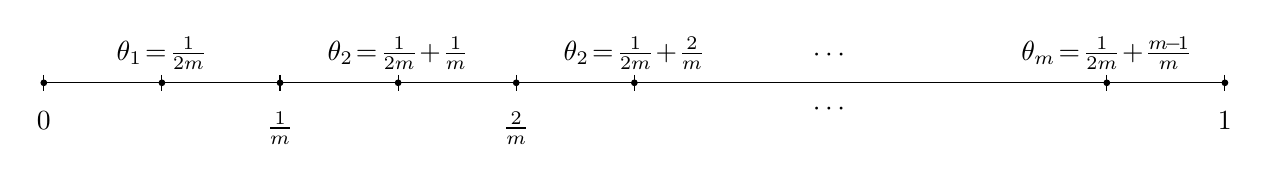
\begin{tikzpicture}[scale=1]
  % Draw horizontal axis
  \draw[-] (0,0) -- (15,0);
  % Mark positions
  \foreach \x/\name in {0/0, 3/$\frac{1}{m}$, 6/$\frac{2}{m}$, 15/1} {
    \draw (\x,0.1) -- (\x,-0.1) node[below=4pt] {\name};
    \filldraw[black] (\x,0) circle (1pt);
  }

  \foreach \x/\name in {1.5/$\theta_1\!=\!\frac{1}{2m}$, 4.5/$\theta_2\!=\!\frac{1}{2m}\!+\!\frac{1}{m}$, 7.5/$\theta_2\!=\!\frac{1}{2m}\!+\!\frac{2}{m}$, 13.5/$\theta_{m}\!=\!\frac{1}{2m}\!+\!\frac{m\!-\!1}{m}$} {
    \draw (\x,0.1) -- (\x,-0.1) node[above=4pt] {\name};
    \filldraw[black] (\x,0) circle (1pt);
  }
  \draw (10, 0) node[above=4pt] {$\cdots$};
  \draw (10, 0) node[below=4pt] {$\cdots$};

\end{tikzpicture}
\caption{Visualization of the discretization on the real line. Ground truth $Y_t$, forecasts $f(t)$ takes values in $\{0, 1/m, ..., 1\}$, and $\theta_i$ are between the grid points.} \label{fig:discretization}
\end{figure}

The following lemma shows that, to control regret uniformly over the class $S_\alpha$, it suffices to control regret on a finite collection of elementary scores $\{S_{\alpha,i}\}_{i=1}^m$. This reduction allows us to replace the original omniprediction objective over $S_\alpha$ with a tractable finite-dimensional problem. Proof is deferred to Appendix \ref{pf:discretize_single_q}.

\begin{lemma}[Discretizing all consistent losses] \label{lem:discretize_single_q}
  For any $\alpha \in (0,1) $, let $S_\alpha$ denote the class of scoring functions with representation \eqref{eq:elem_score_q} with $H([0,1]) \leq 1$.
\[
\sup_{f\in\cf, S\in S_\alpha} \E[S(p(X),Y)] - \E[S(f(X),Y)] 
=
\sup_{f\in\cf, i\in[m]} \E[S_{\alpha,i}(p(X),Y)] - \E[S_{\alpha,i}(f(X),Y)] 
\]
\end{lemma}





\subsection{Omniprediction algorithm and theoretical guarantee} \label{subsec:omni_single_q}
This subsection introduces the omniprediction algorithm that optimizes the losses for all consistent scoring rules for single quantile forecasts. Then, we prove a theoretical upper bound for the omniprediction error of the algorithm.

\begin{algorithm}[h]
  \caption{Single quantile level omniprediction} \label{alg:omni-twoplayer_online_q}
  \begin{algorithmic}[1]
  \State \textbf{Data:} Data stream $\{Y_t\}_{t=1}^T$, Grid size $m \in \mathbb{N}$, Learning rate $\eta > 0$, Base forecasters $\cf = \{f_b\}_{b=1}^{B}$.
  \State For $t=1$,$w_{ib}(t) = \frac{1}{mB}$, for all $i \in [m], b \in [B]$;

  \For{$t = 1, \ldots, T$}
    \State \textbf{1) Make prediction at time $t$}:
    \State $B_k := \sum_{i=1}^{k} \sum_{b=1}^B w_{ib}(t) - \sum_{i=1}^{m} \sum_{b=1}^B w_{ib}(t) \one(\theta_i < f_b(t))$, $\quad k^* = \max\{k: B_k \leq 0\}$
      \State \textbf{Output}
      \makebox[0pt][l]{$\displaystyle
          \hat{P}_t = \frac{B_{k^*+1}}{B_{k^*+1} + |B_{k^*}|}\delta_{\frac{k^*}{m}} +
          \frac{|B_{k^*}|}{B_{k^*+1} + |B_{k^*}|}\delta_{\frac{k^*+1}{m}}$
      } \vspace{-0.1cm}\\
      \State \textbf{2) Update the weights for each $S_{\theta_i}$ and $f_r$}:
          \State $w_{ib}(t+1) = \frac{w_{ib}(t) \exp\bigl(\eta \big(\mathbb{E}_{p \sim \hat{P}_t}[S_{\alpha, i}(p, Y_t)] 
          - S_{\alpha, i}(f_b(t), Y_t)\big)\bigr)}{\sum_{i,b} w_{ib}(t) \exp\bigl(\eta \big(\mathbb{E}_{p \sim \hat{P}_t}[S_{\alpha, i}(p, Y_t)] 
          - S_{\alpha, i}(f_b(t), Y_t)\big)\bigr)}, \quad \forall i \in [m], b \in [B];$ \vspace{-0.1cm}\\
  \EndFor
  \end{algorithmic}
\end{algorithm}



The first part of the algorithm is to produce a prediction at time $t$. Letting $\Delta_m$ denote the set of probability distributions over $\{0, \frac{1}{m}, \frac{2}{m}, ...,1\}$, the prediction $\hat{P}_t$ is computed as the minimax solution to the following program:
\begin{align}\label{eq:minimax_q}
  \hat{P}_t = \arg\min_{P \in \Delta_m} \max_{P_y \in \Delta_m} \sum_{i=1}^{m} \sum_{b=1}^B w_{ib} \,\E_{p\sim P, Y \sim P_y}[S_{\alpha,i}(p,Y) - S_{\alpha,i}(f_b(t),Y)] 
\end{align}
% to obtain a single quantile level forecast version of minimax program solution \eqref{eq:omni-twoplayer-minimax} in Algorithm \ref{alg:omni-twoplayer}.


% Now, we denote forecasts $\{\hat{f}_{\theta_i}\}_{i=0}^{m-1}$ be the forecast that minimizes the losses $\{S_{\alpha, \theta_i}\}_{i=0}^{m-1}$.

Following proposition provides a closed form solution to the minimax program \eqref{eq:minimax_q}, which is incorporated in Algorithm \ref{alg:omni-twoplayer_online_q}, by utilizing the structure of $S_{\alpha, i}$ losses. The proof is deferred to Appendix \ref{pf:minimax_sol_single_q}.

\begin{prop} \label{prop:minimax_sol_single_q}\todo{To add special care on $k^*=m$ case} Define $B_k := \sum_{i=1}^{k} \sum_{b=1}^B w_{ib} - \sum_{i=1}^{m} \sum_{b=1}^B w_{ib} \one(\theta_i < f_b(t))$ and let $k^* = \max\{k: B_k \leq 0\}$. Note that $B_{k^*} \leq 0$ and $B_{k^*+1}>0$. Then, 
\begin{align*}
P^* = \frac{B_{k^*+1}}{B_{k^*+1} + |B_{k^*}|}\delta_{\frac{k^*}{m}} + \frac{|B_{k^*}|}{B_{k^*+1} + |B_{k^*}|}\delta_{\frac{k^*+1}{m}} 
\quad\text{and}\quad
P_y^* = \alpha \delta_0 + (1-\alpha) \delta_1 
\end{align*}
solves equation \eqref{eq:minimax_q}.
\end{prop}

Now, we present the omniprediction error bound for Algorithm \ref{alg:omni-twoplayer_online_q}. The proof is deferred to Appendix \ref{pf:omni-twoplayer_online_q}.

\begin{theorem} \label{thm:omni-twoplayer_online_q}
  For a quantile level $\alpha \in (0,1)$, let $S_\alpha$ denote the class of scoring functions with representation \eqref{eq:elem_score_q} with $H(\R) = 1$ (the set of \textit{all} scoring functions that are consistent for the $\alpha$-level quantile functional under mild regularity conditions). Consider base forecasters $\{f_b\}_{b=1}^B$ that provide $\alpha$-level quantile forecasts $f_b(t)$ at each time step $t \in [T]$. With the target values $Y_t$, forecaster predictions $f_b(t)$ for $t \in [T], b \in [B]$ each taking values in a uniform grid of size $m$, and the learning rate $\eta = \sqrt{\frac{\log mB}{T}}$, the output $\hat{P}_t$ from Algorithm \ref{alg:omni-twoplayer_online_q} achieves the following omniprediction error:
  \begin{align*}
  \sup_{S \in S_\alpha,\, b \in [B]} \frac{1}{T} \sum_{t=1}^T \E_{p \sim \hat{P}(t)} [S(p, Y_t)] - \E[S(f_b(t), Y_t)]
  \leq 2\left(\sqrt{\frac{\log mB}{T}}\right)
  \end{align*}
\end{theorem}


\section{Omniprediction for multiple quantile level forecasts}\label{sec:multi_q}
In this section, we extend the result from Section \ref{sec:single_q} to multiple quantile levels. % To avoid redundancy, we mainly provide online algorithm for omniprediction of multiple quantile level forecasts. Batch version can be straightforwardly extended from the single quantile level case. 
The omniprediction objective we want to minimize is given by
\[
\sup_{S \in \cs,\, f \in \cf} \frac{1}{T} \sum_{t=1}^T \E_{p \sim \hat{P}} [S(p, Y_t)] - \E[S(f_t, Y_t)]
\]
where $\cs$ is the class of \textit{all} scoring functions that are consistent for the multiple quantile levels and $\cf$ is a finite set of competitors or base forecasters.

We follow a similar flow as in Section \ref{sec:single_q}. Section \ref{subsec:decomp_multi_q} discusses the previous result from \cite{fissler2016multiq} on decomposition of scoring function that is consistent for multiple quantile levels. With this result and same discretization scheme from Section \ref{subsec:discretization}, Section \ref{subsec:omni_multi_q} derive a closed-form solution to the multiple quantile level version of minimax program \eqref{eq:minimax_Pt_multi_q} and present the multiple quantile level omniprediction algorithm. Lastly, Section \ref{subsec:separate_multi_q} compares multiple quantile level omniprediction with running separate single quantile level omniprediction for each quantile level.

%Section \ref{subsec:separate_multi_q} shows the cases where post-sorting after solving separate minimax programs for each quantile level works and the cases where it fails, which necessitates the need for solving the minimax program \eqref{eq:omni-twoplayer-minimax} jointly across all quantile levels. 
% Section \ref{subsec:omni_multi_q} provides a closed form solution to the minimax program \eqref{eq:omni-twoplayer-minimax} for multiple quantile levels. Finally, Section \ref{subsec:omni_multi_q_online} puts the results together and provides a sample efficient algorithm for omniprediction of multiple quantile level forecasts.

% \cite{fissler2016multiq} proved that a consistent (proper) loss for multiple quantile levels can be written as a weighted sum of consistent (proper) loss for each quantile levels, under mild regularity conditions.


\subsection{Decomposition of score functions that are consistent for the multiple quantile levels}\label{subsec:decomp_multi_q}
In this subsection, we review the structural characterization of scoring functions that are consistent for multiple quantile levels. \cite{fissler2016multiq} shows that, under mild regularity conditions, any scoring function that is consistent for multiple quantile levels can be written as a weighted sum of scoring functions that are consistent for each individual quantile level. For further details, see Proposition 4.1 and Corollary 4.2 in \cite{fissler2016multiq}. Here, we provide a simplified version of these results that covers only the scope needed for this paper.

\begin{theorem}[Simplified version of Corollary 4.2 in \cite{fissler2016multiq}]
Let $\cf_0$ be the class of the probability measures on the Borel-Lebesgue sets of the real line $\R$. Suppose that $T = (q_{\tau_1}, \ldots, q_{\tau_N}): \cf_0 \to \R^N$ is a functional where each $q_{\tau}$ is a quantile functional at level $\tau$. Then, up to mild regularity conditions, a scoring function $S: \R^N \times \R \to \R$ is strictly consistent for $T$ relative to $\cf_0$ if and only if it is of the form
\begin{align}
    S(x_1, \ldots, x_N, y) = \sum_{n=1}^{N} S_n(x_n, y),
\end{align}
for almost all $(\{x_n\}_{n=1}^N, y) \in \R^N \times \R$, where $S_n: \R \times \R \to \R$, $n \in [N]$, are strictly consistent scoring functions for $q_{\tau_n}$ relative to $\cf_0$.
\end{theorem}

Combined with the decomposition of scoring functions that are consistent for a single quantile level (Theorem \ref{thm:decomp_single_q}), a scoring function that is consistent for multiple quantile levels, $\{\tau_n\}_{n=1}^N$, can be written as a weighted sum of elementary scores of each quantile level. 
\begin{align}\label{eq:multi_q_decomp_raw}
S(x_1, \ldots, x_N, y) = \sum_{n=1}^{N} \int_{-\infty}^{\infty} S_{\tau_n, \theta}(x_n, y) dH_{n}(\theta),
\end{align}
where $H_n$ is a nonnegative measure and $S_{\tau_n, \theta}(x_n, y) = (\one(y<x_n)-\tau_n)(\one(\theta<x_n)-\one(\theta<y))$ for $n \in [N]$ and $\theta \in \R$. 





\subsection{Omniprediction algorithm for multiple quantile levels} \label{subsec:omni_multi_q}
We begin this subsection by introducing the notations and then present the algorithm for multiple quantile level omniprediction. We derive the closed-form solution to the minimax program \eqref{eq:minimax_Pt_multi_q} and present the theorem that provides an upper bound for the omniprediction error of the algorithm.

\paragraph{Notations}
We consider quantile levels $\{\tau_n\}_{n=1}^N$ where $\tau_1 < \tau_2 < ... < \tau_N$ and each base forecasters $f_b$, $b \in [B]$ submits an $N$-length forecast $\{f_b^n\}_{n=1}^N$ for each time step $t=1, ..., T$, where $f_b^n(t)$ corresponds to the $\tau_n$-level quantile estimate from $f_b$ at time $t$.

\paragraph{Discretization}
In a similar vein to the discretization scheme introduced in Section \ref{subsec:discretization}, without loss of generality, we consider the ground truth $Y_t$ and base forecasters $\{f_b^n(t)\}$, $b \in [B], n \in [N]$ to take values in the set $\{0, \frac{1}{m}, ..., 1\}$ and use the same grid of $\{\theta_i\}_{i=1}^{m}$, where $\theta_i = \frac{1}{2m} - \frac{i}{m}$ for $i \in [m]$. Combined with the characterization \eqref{eq:multi_q_decomp_raw}, we can approximate a scoring function that is consistent for multiple quantile levels, $S$, as a weighted sum of elementary scores of each quantile level.
\begin{align*} %\label{eq:multi_q_decomp_discretized}
  S(x_1, \ldots, x_N, y) = \sum_{n=1}^{N} \sum_{i=0}^{m-1} w_i^n \cdot S_{\tau_n, \theta_i}(x_n, y),
\end{align*}
where $w_i^n$ is the weight for the $i$-th grid point of the $n$-th quantile level. 

With the discretization, Algorithm \ref{alg:omni-twoplayer_online_multi_q} presents the multiple quantile level omniprediction algorithm. We abbreviate $S_{\tau_n, \theta_i}$ as $S_{n, i}$.

\begin{algorithm}
  \caption{Two-player game based multiple quantile level online omniprediction} \label{alg:omni-twoplayer_online_multi_q}
  \begin{algorithmic}[1]
  \State \textbf{Data:} Data stream $\{Y_t\}_{t=1}^T$, quantile levels $\tau_1 < \tau_2 < ... < \tau_N$, Grid size $m\in \mathbb{N}$, Learning rate $\eta> 0$, Base forecasters: $\{f_b\}_{b=1}^B$ that outputs $f_b^n(t)$ as $\tau_n$-level quantile estimate at time $t$;
  \State \textit{Initialize:} $w_{ib}^n(1) = \frac{1}{mNB}$, $\forall i \in [m], n \in [N], b \in [B]$;
  \For{$t = 1, \ldots, T$}
    \State \textbf{1) Make prediction at time $t$}:
      \State Define $V_0 = V_N = 0$, $j_0^* = 0$, $j_N^* = m$;
      \State Define $\one_i^n(t) = \{\indi{\theta_i < f_b^n(t)}\}_{b=1}^B \in \R^B$ and $\one_B = (1,..,1)\in \R^B$ for $i \in [m]$ and $n \in [N]$.
      \For{$n=1, \ldots, N-1$}
      \State Compute $V_n(j)$ for $j \in [m]$:
        \(
        V_n(j) = \sum_{i=j+1}^{m} \sum_{s=1}^{n} w_i^s \cdot \one_i^s(t) + \sum_{i=1}^{j} \sum_{s=n+1}^{N}  w_i^s \cdot (\one_B - \one_i^s(t))
        \)
      \State Compute $V_n$ and $j_n^*$:
        \begin{align*}
          V_n = \min_{j \in [m]} V_n(j), \qquad
          j_n^* = \min\left\{j \mid j\in [j_{n-1}^*, m],  V_n(j) = V_n \right\}
        \end{align*}
      \EndFor \vspace{-0.2cm}\\
      \For{$n=1, \ldots, N$}
        \If{$V_n(j_{n-1}^*) = V_n(j_n^*)$}
          \State $\hat{P}_t^n = \delta_{j_{n-1}^*/m}$;
        \Else
          \State Define $B_k := \sum_{i=1}^{k} w_i^n(t) \cdot \one_B - \sum_{i=1}^{m}w_i^n(t) \cdot \one_i^n(t)$
          \State Find $j_{n-1}^* \leq k_n < j_n^*$ s.t. $B_{k_n} < V_{n-1} - V_n \leq B_{k_n+1}$ (Existence proved in Lemma \ref{lem:Pn_def})
          \State $\hat{P}_t^n = (1-C_n)\delta_{k_n/m} + C_n\delta_{((k_n+1)/m)}$, where $C_n = \left( V_{n-1} - V_n - B_{k_n} \right) / (w_{k_n}^n \cdot \one_B)$
        \EndIf
      \EndFor
      \State \textbf{Output} $\hat{P}_t = \{\hat{P}_t^n\}_{n=1}^N$;  \vspace{-0.1cm}\\
      \State \textbf{2) Update the weights for each $S_{n,i} = (\one(y<x)-\tau_n)(\one(\theta_i<x)-\one(\theta_i<y))$}:
          \State $w_{ib}^n(t+1) 
          = \frac{w_{ib}^n(t) \exp\bigl(\eta \big(\mathbb{E}_{p \sim \hat{P}_t^n}[S_{n,i}(p, Y_t)] 
          - S_{n,i}(\hat{f}_i^n(t), Y_t)\big)\bigr)}
          {\sum_{i=1}^{m} \sum_{n=1}^N \sum_{b=1}^B w_{ib}^n(t) \exp\bigl(\eta \big(\mathbb{E}_{p \sim \hat{P}_t^n}[S_{n,i}(p, Y_t)] - S_{n,i}(\hat{f}_b^n(t), Y_t)\big)\bigr)}, \quad \forall i \in [m], n \in [N], b \in [B];$ \vspace{-0.1cm}\\
  \EndFor
  \end{algorithmic}
\end{algorithm}



%%% HERE Apr. 13

As in the case of single quantile level omniprediction, the first part of the algorithm is to make a prediction at time $t$. $\hat{P}_t$ computed here is a minimax solution for the following minimax program, which hasone additional dimension compared to the single quantile level case:

\[
\min_{\tilde{P} \in \cd(\Delta_m)} \max_{P_y \in \Delta_m} \sum_{n=1}^N \sum_{i=0}^{m-1} \sum_{b=1}^F w_{ib}^n \E_{P\sim \tilde{P}, Y \sim P_y}[S_i^n(q_{\tau_n}(P),Y) - S_i^n(f_b^n(t),Y)],
\]
where $q_{\tau_n}(P)$ is the $\tau_n$-level quantile of $P$ and $S_i^n(x, Y) = (\one(Y < x)-\tau_n)(\one(\theta_i<x)-\one(\theta_i<Y))$ as defined previously. We can rewrite the program as follows:
\begin{align}\label{eq:minimax_Pt_multi_q}
\min_{P_1, P_2, ..., P_N \in \Delta_m} \max_{P_y \in \Delta_m} \sum_{n=1}^N \sum_{i=0}^{m-1} \sum_{b=1}^F w_{ib}^n \E_{p_n \sim P_n
, Y \sim P_y}[S_i^n(p_n,Y) - S_i^n(f_b^n(t),Y)],
\end{align}
with the constraint that the joint distribution ($P_1, P_2, ..., P_N$) always satisfies the ordering of the samples $p_1 \leq p_2 \leq ... \leq p_N$. During derivation of the closed-form solution, we also prove that our closed-form solution satisfies this monotonicity constraint.


\begin{lemma}\label{lem:jn_sort}
Define the quantity $V_n$ for $n \in [N-1]$ as
\begin{align} \label{eq:Vn_def}
V_n := \min_{j \in [m]} \left( \sum_{i=j}^{m-1} \sum_{s=1}^{n} \sum_{b=1}^F w_{ib}^s \indi{\theta_i < f_b^s(t)} + \sum_{i=0}^{j-1} \sum_{s=n+1}^{N}  \sum_{b=1}^F w_{ib}^s (1 - \indi{\theta_i < f_b^s(t)})\right) \geq 0
\end{align}
and $V_0 = V_N := 0$.
Let $J_n^*$ be the set of indices $j \in [m]$ that minimizes the $V_n$. 
\smallskip \\
Then, there exists a sorted sequence $0=j_0^* \leq j_1^* \leq ... \leq j_{N-1}^* \leq j_N^* = m$ such that $j_n^* \in J_n^*$ for $n \in [N-1]$.
\end{lemma}

\begin{proof}
Define $w_i^s := (w_{1b}^s, ..., w_{Fb}^s) \in \R^F$, $\one_i^s = (\indi{\theta_i < f_1^s(t)}, ..., \indi{\theta_i < f_F^s(t)}) \in \R^F$, and $\one_F = (1, ..., 1) \in \R^F$. Then, $V_n$ can be rewritten as
\[
V_n = \min_{j \in [m]} \left( \sum_{i=j}^{m-1} \sum_{s=1}^{n} w_i^s \cdot \one_i^s + \sum_{i=0}^{j-1} \sum_{s=n+1}^{N}  w_i^s \cdot (\one_F - \one_i^s) \right).
\]
Suppose there exists a pair of indices $n, n+1$ such that $j_n^* > j_{n+1}^*$. Using the definition of $V_n$, we have 
\begin{align*}
j_n^* &= \argmin_{j \in [m]} \left( \sum_{i=j}^{m-1} \sum_{s=1}^{n} w_i^s \cdot \one_i^s + \sum_{i=0}^{j-1} \sum_{s=n+2}^{N}  w_i^s \cdot (\one_F - \one_i^s) + \sum_{i=0}^{j-1} w_i^{n+1} \cdot (\one_F - \one_i^{n+1})\right) \\
j_{n+1}^* &= \argmin_{j \in [m]} \left( \sum_{i=j}^{m-1} \sum_{s=1}^{n+1} w_i^s \cdot \one_i^s + \sum_{i=0}^{j-1} \sum_{s=n+2}^{N}  w_i^s \cdot (\one_F - \one_i^s) + \sum_{i=j}^{m-1} w_i^{n+1} \cdot \one_i^{n+1}\right).
\end{align*}
Two expressions share the first two terms and differ in the last term. We abbreviate these terms as following:
\begin{align*}
C_j & := \sum_{i=j}^{m-1} \sum_{s=1}^{n} w_i^s \cdot \one_i^s + \sum_{i=0}^{j-1} \sum_{s=n+2}^{N}  w_i^s \cdot (\one_F - \one_i^s) \\
D_j & := \sum_{i=0}^{j-1} w_i^{n+1} \cdot (\one_F - \one_i^{n+1}) \\
E_j & := \sum_{i=j}^{m-1} w_i^{n+1} \cdot \one_i^{n+1}.
\end{align*}
Note that $D_j$ is non-decreasing in $j$ and $E_j$ is non-increasing in $j$.
Since $j_n^*$ and $j_{n+1}^*$ are the indices that minimize the $V_n$ and $V_{n+1}$, respectively, we have $C_{j_n^*} + D_{j_n^*} \leq C_{j_{n+1}^*} + D_{j_{n+1}^*}$ and $C_{j_n^*} + E_{j_n^*} \geq C_{j_{n+1}^*} + E_{j_{n+1}^*}$. This implies that 
\[
E_{j_{n+1}^*} - E_{j_n^*} \leq C_{j_n^*} - C_{j_{n+1}^*} \leq D_{j_{n+1}^*} - D_{j_n^*}.
\]
Because of the monotonicity of $D_j$ and $E_j$ and the assumption that $j_n^* > j_{n+1}^*$, the leftmost term should be non-negative and the rightmost term should be non-positive. Therefore, we obtain 
\[
C_{j_n^*} - C_{j_{n+1}^*} = D_{j_n^*} - D_{j_{n+1}^*} = E_{j_n^*} - E_{j_{n+1}^*} = 0 \quad \Rightarrow j_{n+1}^* \in J_n^*, \,\, j_n^* \in J_{n+1}^*.
\]
By choosing $j_{n+1}^*$ as a minimizer of $V_n$ and $j_n^*$ as a minimizer of $V_{n+1}$, we resolve the unsorted pair of indices. Repeating this process yields a sorted sequence $0=j_0^* \leq j_1^* \leq ... \leq j_{N-1}^* \leq j_N^* = m$ and this proves the existence of sorted sequence.
\\
Due to its existence, we can simply obtain a sorted sequence by choosing $j_n^* = \min J_n^*$ for all $n \in [N]$.
\end{proof}

\begin{lemma} \label{lem:Pn_def}
Given a sorted sequence $0=j_0^* \leq j_1^* \leq ... \leq j_{N-1}^* \leq j_N^* = m$, there exists a distribution $P_n^*$ for $n \in [N]$ of the form
\begin{align}\label{eq:Pn_def}
P_n^* = (1-C_n)\delta_{k_n / m} + C_n\delta_{(k_n+1)/m},
\end{align}
such that 
\begin{enumerate}
  \item $j_{n-1}^* \leq k_n$
  \item $k_n < j_n^*$ if $j_{n-1}^* \neq j_n^*$ and $k_n = j_n^*$ with $C_n=0$ if $j_{n-1}^* = j_n^*$.
  \item The support of $P_n^*$ is contained in $[j_{n-1}^*/m, j_n^*/m]$.
  \item $\E_{p_n \sim P_n^*} \left[ \sum_{i=0}^{m-1} \sum_{b=1}^F w_{ib}^n \left( \indi{\theta_i < p_n} - \indi{\theta_i < f_b^n(t)} \right) \right] = V_{n-1}-V_n$.
\end{enumerate}
\end{lemma}
\begin{proof}
We again use the notations used in proof of Lemma \ref{lem:jn_sort}. We define a function $V_n(\cdot)$ as following:
\begin{align}\label{eq:Vn_j_def}
V_n(j) = \sum_{i=j}^{m-1} \sum_{s=1}^{n} w_i^s \cdot \one_i^s + \sum_{i=0}^{j-1} \sum_{s=n+1}^{N}  w_i^s \cdot (\one_F - \one_i^s)  \quad \forall j \in [m], n \in [N].
\end{align}
Note that the quantity $V_n$ defined in Lemma \ref{lem:jn_sort} is equal to $V_n(j_n^*)$ for all $n \in [N-1]$ and that $V_n(j) \geq V_n(j_n^*)$ for all $j \in [m]$.
\\
With the fact that $\indi{\theta_i < k/m} = \indi{i < k}$, the last condition in the lemma statement is equivalent to 
\begin{align*} 
& \E_{p_n \sim P_n^*} \left[ \sum_{i=0}^{m-1} \sum_{b=1}^F w_{ib}^n \left( \indi{\theta_i < p_n} - \indi{\theta_i < f_b^n(t)} \right) \right] \nonumber\\
& = (1-C_n) \sum_{i=0}^{m-1} \sum_{b=1}^F w_{ib}^n \left( \indi{i < k_n} - \indi{\theta_i < f_b^n(t)} \right) + C_n \sum_{i=0}^{m-1} \sum_{b=1}^F w_{ib}^n \left( \indi{i < k_n+1} - \indi{\theta_i < f_b^n(t)} \right) \nonumber\\
& = (1-C_n) \sum_{i=0}^{m-1} w_{i}^n \cdot \left( \indi{i < k_n} \one_F - \one_i^n \right) + C_n \sum_{i=0}^{m-1} w_{i}^n \cdot \left( \indi{i < k_n+1} \one_F - \one_i^n \right) \nonumber\\
& = \sum_{i=0}^{k_n-1} w_i^n \cdot \one_F + C_n w_{k_n}^n \cdot \one_F - \sum_{i=0}^{m-1} w_i^n \cdot \one_i^n \\
& = V_{n-1} - V_n.  
\end{align*}
The last equality is equivalent to 
\begin{align}
\sum_{i=0}^{k_n-1} w_i^n \cdot \one_F + C_n w_{k_n}^n \cdot \one_F 
= \sum_{i=0}^{m-1} w_i^n \cdot \one_i^n + V_{n-1} - V_n 
= \sum_{i=0}^{j_{n-1}^*-1} w_i^n \cdot \one_F + V_n(j_{n-1}^*) - V_n(j_n^*), \label{eq:Pn_eq}
\end{align}
where we used the fact that $\sum_{i=0}^{m-1} w_i^n \cdot \one_i^n + V_{n-1}(j) = \sum_{i=0}^{j-1} w_i^n \cdot \one_F + V_n(j)$ with $j=j_{n-1}^*$.
\smallskip \\
Now we divide the cases into three cases. 
First, consider the case where $j_{n-1}^* = j_n^*$. In this case, simply $k_n = j_{n-1}^*$ with $C_n=0$ satisfies the equation \eqref{eq:Pn_eq}. Therefore, $P_n^* = \delta_{j_{n-1}^*/m}$ satisfies the conditions.
Second, consider the case where $j_{n-1}^* < j_n^*$ but $V_n(j_{n-1}^*) = V_n(j_n^*)$. $k_n = j_{n-1}^*$ with $C_n=0$ again satisfies the equation \eqref{eq:Pn_eq} and $k_n = j_{n-1}^* < j_n^*$ in this case.
Lastly, consider the case where $V_n(j_{n-1}^*) > V_n(j_n^*)$. We have 
\begin{align*}
  \sum_{i=0}^{j_{n-1}^*-1} w_i^n \cdot \one_F
  & < \sum_{i=0}^{j_{n-1}^*-1} w_i^n \cdot \one_F + V_n(j_{n-1}^*) - V_n(j_n^*) \\
  & = \sum_{i=0}^{m-1} w_i^n \cdot \one_i^n - V_n + V_{n-1} \\
  & = \sum_{i=0}^{j_{n}^*-1} w_i^n \cdot \one_F + V_{n-1}(j_{n-1}^*) - V_{n-1}(j_n^*) 
  \leq \sum_{i=0}^{j_{n}^*-1} w_i^n \cdot \one_F,
\end{align*}

where two equalities used the fact that $\sum_{i=0}^{m-1} w_i^n \cdot \one_i^n + V_{n-1}(j) = \sum_{i=0}^{j-1} w_i^n \cdot \one_F + V_n(j)$ with $j=j_n^*$ on the second term of the equation \eqref{eq:Pn_eq}.
This implies that there exists a $j_{n-1}^* \leq k_n < j_n^*$ such that 
\begin{align*}
  \sum_{i=0}^{k_n} w_i^n \cdot \one_F \geq \sum_{i=0}^{m-1} w_i^n \cdot \one_i^n - V_n + V_{n-1} \quad \text{and} \quad \sum_{i=0}^{k_n-1} w_i^n \cdot \one_F < \sum_{i=0}^{m-1} w_i^n \cdot \one_i^n - V_n + V_{n-1}.
\end{align*}
With such $k_n$, we define $P_n^*$ with $C_n = \frac{1}{w_{k_n}^n \cdot \one_F} \left( \sum_{i=0}^{m-1} w_i^n \cdot \one_i^n - V_n + V_{n-1} - \sum_{i=0}^{k_n-1} w_i^n \cdot \one_F \right)$ and this satisfies the conditions since $k_n+1 \leq j_n^*$.
\end{proof}





Now we provide the solution to the minimax program \eqref{eq:omni-twoplayer-minimax}.
\begin{theorem}\label{thm:minimax_negative_multi_q}
Given quantile levels $\tau_1 < \tau_2 < ... < \tau_N$, quantile forecasts $\hat{f}_i^n$ for $i =0,...,m\!-\!1$ and $n \in [N]$, define $V_n$ $n \in [N-1]$ as in equations \eqref{eq:Vn_def}, with $V_0 = V_N := 0$. Let $\{j_n^*\}_{n=1}^{N-1}$ be a sorted sequence of indices that minimizes the $V_n$ for $n \in [N-1]$ with $j_0^* = 0$ and $j_N^* = m$ where the existence of the sequence is guaranteed by Lemma \ref{lem:jn_sort}. 
\smallskip \\
Then, $P_n^*$ for $n \in [N]$ given by \eqref{eq:Pn_def} with 
\[
P_y^* = \tau_1 \delta_0 + (1-\tau_N)\delta_1 + \sum_{n=1}^{N-1}(\tau_{n+1}-\tau_n)\delta_{j_t^*/m}
\]
solves the minimax program \eqref{eq:omni-twoplayer-minimax} and the value of the minimax program is 
\[
-\sum_{n=1}^{N-1}(\tau_{n+1}-\tau_n)V_n \leq 0.
\]

% Then, the value of the minimax program is $-\sum_{t=1}^{N-1}(\tau_{t+1}-\tau_t)V_t \leq 0$ and the solution is given by 
% \begin{align*}
%   P_y^* &= \tau_1 \delta_0 + (1-\tau_N)\delta_1 + \sum_{t=1}^{N-1}(\tau_{t+1}-\tau_t)\delta_{j_t^*/m} \\
%   P_t^* &= C_t \delta_{\underline{k_t^*}/m} + (1-C_t) \delta_{(\underline{k_t^*}+1)/m}, \quad t \in [N],
% \end{align*}
% where
% \begin{align*}
%   \underline{k_t^*} &= \min\left\{k \mid \sum_{i=0}^k w_i^t \geq \sum_{i=0}^{m-1} w_i^t \indi{\theta_i < \hat{f}_i^t} - V_t + V_{t-1} \right\} \\
%   \overline{k_t^*} &= \min\left\{k \mid \sum_{i=0}^k w_i^t > \sum_{i=0}^{m-1} w_i^t \indi{\theta_i < \hat{f}_i^t} - V_t + V_{t-1} \right\} \\
%   C_t & = \frac{1}{w_{\underline{k_t^*}}^t} \left( \sum_{i=0}^{\underline{k_t^*}} w_i^t - \left(\sum_{i=0}^{m-1} w_i^t \indi{\theta_i < \hat{f}_i^t} - V_t + V_{t-1}\right)\right),
% \end{align*}
% for $t \in [N]$ with $V_0 = V_N := 0$.

% Moreover, for any $j_t^*$ that achieves the minimum in \eqref{eq:Vt_def}, it holds that $\underline{k_t^*} < j_t^* \leq \overline{k_{t+1}^*}$, \sout{which implies that $P_t^*$ is stochastically smaller than $P_{t+1}^*$}. {\color{red} I'm confident that $\underline{k_t^*} \leq \underline{k_{t+1}^*}$ also holds, so that $\underline{k_t^*}$ doesn't have crossing issue.}
\end{theorem}
\begin{proof}
Denote the minimax objective function by 
\[O(\{P_n\}_{n=1}^N, P_y) = \sum_{n=1}^N \sum_{i=0}^{m-1} \sum_{b=1}^F w_{ib}^n \E_{p_n \sim P_n, Y \sim P_y}[S_{\tau_n,\theta_i}(p_n,Y) - S_{\tau_n,\theta_i}(f_b^n(t),Y)].
\]
In a similar vein to the proof of Lemma \ref{lem:minimax_sol_single_q}, we show $O(\{P_n^*\}_{n=1}^N, P_y^*) = \max_{P_y} O(\{P_n^*\}_{n=1}^N, P_y)$ then show $O(\{P_n^*\}_{n=1}^N, P_y^*) = \min_{P_n \in \Delta_m, n\in[N]} O(\{P_n\}_{n=1}^N, P_y^*)$.

Following the decomposition \eqref{eq:oppy_q}, $O(\{P_n\}_{n=1}^N, P_y)$ can be written as
\[
O(\{P_n\}_{n=1}^N, P_y) = \sum_{n=1}^N \sum_{i=0}^{m-1} \sum_{b=1}^F w_{ib}^n \E_{p_n \sim P_n, Y \sim P_y}[\one(Y \leq \theta_i < p_n) - \tau_n \one(\theta_i<p_n) - \one(Y \leq \theta_i < f_b^n(t))] + C_n,
\]
where $C_n =\tau_n \sum_{i=0}^{m-1} \sum_{b=1}^F w_{ib}^n \indi{\theta_i < f_b^n(t)}$ which does not depend on $P_n$ or $P_y$.

Using this decomposition, we prove $O(\{P_n^*\}_{n=1}^N, P_y^*) = \max_{P_y} O(\{P_n^*\}_{n=1}^N, P_y)$. Let $P_y(\frac{j}{m})=p_{yj}$ for $j=0,...,m$. Then, again using the notation from the proof of Lemma \ref{lem:jn_sort}, $O(\{P_n^*\}_{n=1}^N, P_y)$ is rephrased as the following:
\begin{align}\label{eq:O_Pstar_Py_decomp}
O(\{P_n^*\}_{n=1}^N, P_y) 
& = \sum_{n=1}^N \E_{p_n \sim P_n^*} \left[\sum_j p_{yj} \sum_{i=j}^{m-1} w_i^n \cdot \left( \indi{\theta_i < p_n} \one_F - \one_i^n \right)\right] + C(P_n^*),
\end{align}
where $C(P_n^*) = - \tau_n \E_{p_n \sim P_n^*} \sum_{i=0}^{m-1} w_i^n \cdot (\indi{\theta_i < p_n} \one_F - \one_i^n)$ only depends on $P_n^*$ and does not depend on $P_y$.

Plugging in $P_n^*$ and abbreviating $\indi{\theta_i < \hat{f}_i^n}$ with $\one_i^n$, the summand can be expressed as 
\begin{align*}
A_j^n := \E_{p_n \sim P_n^*} & \left[\sum_{i=j}^{m-1} w_i^n \cdot \left( \indi{\theta_i < p_n} \one_F - \one_i^n\right)\right] 
= \begin{cases}
-\sum_{i=0}^{j-1} w_i^n \cdot (\one_F-\one_i^n) - V_n + V_{n-1} & \quad j \leq k_n^* \\
- \sum_{i=j}^{m-1} w_i^n \cdot \one_i^n & \quad j > k_n^* \\
\end{cases} 
\end{align*}

This leads to 
\begin{align*}
A_j & := \sum_{n=1}^N A_j^n \\
&= \begin{cases}
-\sum_{n=1}^N \sum_{i=0}^{j-1} w_i^n \cdot (\one_F-\one_i^n) + V_0 & \quad j \leq k_1 \\
-\sum_{n=1}^\nu \sum_{i=j}^{m-1} w_i^n \cdot \one_i^n - \sum_{n=\nu+1}^{N} \sum_{i=0}^{j-1} w_i^n \cdot (\one_F-\one_i^n) + V_\nu & \quad  j \in (k_\nu, k_{\nu+1}], \,\, \nu \in [N-1] \\
-\sum_{n=1}^N \sum_{i=j}^{m-1} w_i^n \cdot \one_i^n + V_N & \quad j > k_N
\end{cases}
\end{align*}
Notice that $A_j$ is non-increasing on $j \leq k_1$ and non-decreasing on $j > k_N$. $A_0 = 0$ and $A_m = 0$ is the maximum value of $A_j$ in these ranges, respectively. Next, observe that $A_j \leq 0$ for all $j=0,1,...,m$ since $V_n$ is the minimum value that $\sum_{\nu=1}^n \sum_{i=j}^{m-1} w_i^n \cdot \one_i^\nu + \sum_{\nu=n+1}^{N} \sum_{i=0}^{j-1} w_i^{\nu} \cdot (\one_F-\one_i^{\nu})$ can achieve by its definition. It suffices to show that $A_{j_n^*} = 0$ for $n \in [N-1]$ since $P_y^*$ only puts mass on these points. Note that $A_{j_0} = A_0 = 0$ and $A_{j_N} = A_m = 0$.

From the first and second condition in the statement of Lemma \ref{lem:Pn_def}, we have $k_\nu < j_\nu^* \leq k_{\nu+1}$ if $j_{\nu-1}^* \neq j_\nu^*$ and $j_{\nu-1}^* = j_\nu^*= k_\nu$ if $j_{\nu-1}^* = j_\nu^*$, for $\nu \in [N-1]$. In the former case, we obtain $A_{j_\nu^*} = 0$ from $k_\nu < j \leq k_{\nu+1}$ case in the definition of $A_j$ above. In the latter case, $j_\nu^* = k_\nu$ does not fall into the range $(k_\nu, k_{\nu+1}]$. Still, from $k_{\nu-1} < j \leq k_{\nu}$ case ($j \leq k_1$ case if $\nu=1$) in the definition of $A_j$ , we have
\begin{align*}
A_{j_n^*} 
& = -\sum_{n=1}^{\nu-1} \sum_{i=j}^{m-1} w_i^n \cdot \one_i^n - \sum_{n=\nu}^{N} \sum_{i=0}^{j-1} w_i^n \cdot (\one_F - \one_i^n) + V_{\nu-1} \\
& =  - V_{\nu-1}(j_n^*) + V_{\nu-1} = -V_{\nu-1}(j_{n-1}^*) + V_{\nu-1} = 0,
\end{align*}
where $V_n(j)$ is defined as equation \eqref{eq:Vn_j_def}. Therefore, $A_{j_n^*} = 0$ for all $n \in [N-1]$ and $O(\{P_n^*\}_{n=1}^N, P_y^*) = \max_{P_y} O(\{P_n^*\}_{n=1}^N, P_y)$.

Next, we show that $O(\{P_n^*\}_{n=1}^N, P_y^*) = \min_{P_n \in \Delta_m, n\in[N]} O(\{P_n\}_{n=1}^N, P_y^*)$. This follows directly from the consistency of $S_{\tau,\theta_i}$ losses and the third condition in Lemma \ref{lem:Pn_def}. Any point in the support of $P_n^*$ is $\tau_n$-level quantile of $P_y^*$ since $P_y(Y \leq j_{n-1}^*/m) = \tau_n$ and $P_y(Y \geq j_n^*/m) = \tau_n$.

Lastly, we compute the value of the minimax program. Decomposition \eqref{eq:O_Pstar_Py_decomp} can be rewritten as 
\[
O(\{P_n^*\}_{n=1}^N, P_y) = \sum_{j} p_{yj} A_j + \sum_{n=1}^N C(P_n^*).
\]
Since $P_Y^*$ only puts mass on points $j/m$ such that $A_j = 0$, plugging in $P_y^*$ into the equation above yields
\begin{align*}
O(\{P_n^*\}_{n=1}^N, P_y^*) 
&= \sum_{n=1}^N C(P_n^*) = -\sum_{n=1}^N \tau_n \E_{p_n \sim P_n^*} \sum_{i=0}^{m-1} w_i^n \cdot (\indi{\theta_i < p_n}\one_F - \one_i^n) \\
&  = -\sum_{n=1}^N \tau_n (V_{n-1} - V_n) = -\sum_{n=1}^{N-1}(\tau_{n+1}-\tau_n)V_n \leq 0,
\end{align*}
where the second from the last equality used the fourth condition in Lemma \ref{lem:Pn_def}.
\end{proof}


\subsection{Sample efficient algorithm for omniprediction of multiple quantile level forecasts}\label{subsec:omni_multi_q_online}

  


\begin{theorem}
  \label{thm:omni-twoplayer_online_multi_q}
  For a set of quantile levels $\tau_1 < \tau_2 < ... < \tau_N$, let $\cs$ denote the class of scoring functions with representation \eqref{eq:multi_q_consistent_loss} with positive measures $\{H_{\tau_n}\}_{n=1}^N$ such that $H_{\tau_n}(\R) \leq 1, \forall n \in [N]$ (the set of \textit{all} scoring functions that are consistent for the multiple quantile levels under mild regularity conditions). Consider a class of competitors $\cf$ where each forecaster $f \in \cf$ provides $\{\tau_n\}_{n=1}^N$-level quantile forecasts $\{f^n(t)\}_{n=1}^N$. With the target values $Y_t$, forecaster predictions $f^n(t)$ for $t \in [T], n \in [N], f \in \cf$ each taking values in a discretized grid of size $m$, and the learning rate $\eta_w = O(\sqrt{\frac{\log (mN)}{T}})$ and $\eta_f = O(\sqrt{\frac{\log |\cf|}{T}})$, the output $\hat{P}_t = \{\hat{P}_t^n\}_{n=1}^N$ from Algorithm \ref{alg:omni-twoplayer_online_multi_q} achieves the following omniprediction error:
  \begin{align*}
  \sup_{S \in \cs,\, f \in \cf} \frac{1}{T} \sum_{n=1}^N \sum_{t=1}^T \E_{p \sim \hat{P}_t^n} [S(p, Y_t)] - \E[S(f^n(t), Y_t)]
  \leq O\left(\sqrt{\frac{\log mN|\cf|}{T}}\right)
  \end{align*}
\end{theorem}

\begin{proof}
  Straightforward extension of Theorem \ref{thm:omni-twoplayer_online_q}, using theorem \ref{thm:minimax_negative_multi_q}.
\end{proof}












\subsection{Separate omniprediction for each quantile level}\label{subsec:separate_multi_q}
\cite{fakoor2023flexible} showed that post-sorting and isotonic projection decrease the loss for \textbf{unweighted} weighted sums of pinball losses at different quantile levels. Unfortunately, post-sorting does not achieve the same for \textbf{weighted} sums of pinball losses.

Define the pinball loss at quantile level $\tau$ as $\rho_\tau(x) := \tau x\indi{x \geq 0} +(1-\tau)|x|\indi{x < 0} = (\tau - \indi{x < 0})x$. Then define the loss function 
\[
\ell(x_1, x_2) := \E_Y [w_\alpha \rho_\alpha (y-x_1) + w_\beta \rho_\beta (y-x_2)].
\] 
Consider the case $\alpha < \beta$. We would like $\ell(x_1, x_2) - \ell(x_2, x_1) \geq 0$ for $x_1 > x_2$. 
\paragraph{Counterexample} Let $Y \sim \text{Ber}(1/2)$ and $0 < x_2 < x_1 < 1$. Then, 
\begin{align*}
\ell(x_1, x_2) - \ell(x_2, x_1) 
& = w_\alpha \E_Y \left[(\alpha - \indi{y < x_1})(y-x_1) - (\alpha - \indi{y < x_2})(y-x_2)\right] + \\ 
& \qquad w_\beta \E_Y \left[(\beta - \indi{y < x_2})(y-x_2) - (\beta - \indi{y < x_1})(y-x_1) \right] \\
& = w_\alpha (\alpha - 1/2)(x_2 - x_1) + w_\beta (\beta - 1/2)(x_1 - x_2) \\
& = (x_1 - x_2)(w_\beta (\beta - 1/2) - w_\alpha (\alpha - 1/2))
\end{align*}
Note that the second equality uses the fact that $\indi{y < x_1} = \indi{y < x_2}$. When $\alpha$ and $\beta$ lie on the same side of $1/2$, there exist $(w_\alpha, w_\beta)$ for which the improvement in loss becomes negative.
Conversely, if $(w_\alpha, w_\beta)$ does not satisfy any of the above conditions, then there exists $(Y, x_1, x_2)$ such that post-sorting increases the loss.

\smallskip
If we solve the minimax program \textbf{separately for each quantile level}, quantile crossing may occur (or maybe NOT due to the structure of $f(X)$ that it is a valid probability forecast and thus no quantile crossing occurs). Unfortuately, the following proposition shows that post-sorting does not always reduce loss for \textbf{unequally} weighted sums of pinball losses.

\subsubsection{Characterizaion of weighted quantile loss that post-sorting does decrease the loss}
\begin{prop}
As above, define a weighted quantile loss as
\[
\ell(x_1, x_2) := \E_Y [w_\alpha \rho_\alpha (y-x_1) + w_\beta \rho_\beta (y-x_2)].
\]
If $(w_\alpha, w_\beta)$ satisfies one of the following conditions, then post-sorting does not increase the loss:
\begin{enumerate}
  \item $w_\alpha = w_\beta$
  \item $w_\alpha < w_\beta$ and $(1-\alpha)w_\alpha \geq (1-\beta)w_\beta$
  \item $w_\alpha > w_\beta$ and $\beta w_\beta \geq \alpha w_\alpha$.
\end{enumerate}
Conversely, if $(w_\alpha, w_\beta)$ does not satisfy any of the above conditions, then there exists $(Y, x_1, x_2)$ such that post-sorting increases the loss.
\end{prop}

\begin{proof}
\begin{align*}
\ell(x_1, x_2) - \ell(x_2, x_1) 
& = w_\alpha \E_Y \left[(\alpha - \indi{y < x_1})(y-x_1) - (\alpha - \indi{y < x_2})(y-x_2) \right] + \\ 
& \qquad w_\beta \E_Y \left[(\beta - \indi{y < x_2})(y-x_2) - (\beta - \indi{y < x_1})(y-x_1) \right] \\
& = w_\alpha E_Y \left[\left\{-\alpha(x_1 - x_2) + \indi{y < x_1}x_1 - \indi{y < x_2}x_2 - \indi{x_2 \leq y < x_1}y \right\}\right] + \\
& \qquad w_\beta E_Y \left[ \left\{\beta(x_1 - x_2) + \indi{y < x_2}x_2 - \indi(y < x_1)x_1 + \indi{x_2 \leq y < x_1}y \right\} \right] \\
& = \E_Y \left[\left\{-\alpha(x_1 - x_2) + \indi{x_2 \leq y < x_1}(x_1 - y) + \indi{y < x_2}(x_1 - x_2)\right\} \right] w_\alpha + \\
& \qquad \E_Y \left[\left\{\beta(x_1 - x_2) - \indi{x_1 \leq y < x_2}(x_1 - y) - \indi{y < x_2}(x_1 - x_2)\right\} \right] w_\beta 
\end{align*}
Denote the coefficient of $w_\alpha, w_\beta$ as $c_\alpha, c_\beta$ respectively. Notice that $c_\alpha + c_\beta = (\beta-\alpha)(x_1 - x_2) > 0$. Therefore $\ell(x_1, x_2) - \ell(x_2, x_1) > 0$ if $w_\alpha = w_\beta$ (Condition I).
Denote $A = \P(y < x_2)$, $B = \P(x_2 \geq y < x_1)$ and observe that $\E_Y \indi{x_2 \geq y < x_1}(x_1 - y) \in [0, B(x_1 - x_2)]$.
We now consider Condition II: $w_\alpha < w_\beta$ and $(1-\alpha)w_\alpha \geq (1-\beta)w_\beta$. 
\begin{align*}
\ell(x_1, x_2) - \ell(x_2, x_1) 
& = \left(w_\alpha(A-\alpha) + w_\beta(\beta-A)\right)(x_1 - x_2) - (w_\beta - w_\alpha)\E_Y \indi{x_2 \leq y < x_1}(x_1 - y) \\
& \geq -(w_\beta - w_\alpha)A + \beta w_\beta - \alpha w_\alpha - (w_\beta - w_\alpha)B(x_1 - x_2) \\
& \geq -(w_\beta - w_\alpha)A + (w_\beta - w_\alpha) - (w_\beta - w_\alpha)B(x_1 - x_2) \\
& \geq (w_\beta - w_\alpha)(1-A-B)(x_1 - x_2) \geq 0.
\end{align*}
Note that $\beta w_\beta - \alpha w_\alpha \geq w_\beta - w_\alpha$ follows from the condition and $A+B = \P(Y < x_1) \leq 1$.
Condition III is similar.
{\color{red} If we put this propoisition in the paper, add constructing counterexample for $(w_\alpha, w_\beta)$ that does not satisfy any of the above conditions.}
\end{proof}

Alternatively, we prove another class of loss functions where post-sorting does not increase the loss. Due to \cite{fissler2016multiq}, a loss function that is consistent for multiple quantile levels can be written as a weighted sum of consistent (proper) loss for each quantile levels, under mild regularity conditions:
\begin{align} \label{eq:multi_q_consistent_loss}
\ell(\{x_i\}_{i=1}^N, y) = \E_Y \sum_{i=1}^{N} w^i (\indi{y < x_i} - \tau_i)(g_i(x_i) - g_i(y)),  
\end{align}
where $g_i$ is a non-decreasing function.
\begin{prop}
If a loss function $\ell$ defined as \eqref{eq:multi_q_consistent_loss} satisfies $w_i = w$ and $g_i(x) = g(x)$ for all $i \in [N]$, then post-sorting does not increase the loss.
\end{prop}
\begin{proof}
Due to additivity of the loss function, it suffices to show $\ell(x_1, x_2, y) - \ell(x_2, x_1, y) \geq 0$ for $x_1 > x_2$ where $x_i$ corresponds to the $\tau_i$-level quantile estimate. Without loss of generality, assume $w=1$.
\begin{align*}
\ell(x_1, x_2, y) & - \ell(x_2, x_1, y) 
= \E_Y [ (\indi{y < x_1} - \tau_1)(g_1(x_1) - g_1(y)) - (\indi{y < x_2} - \tau_1)(g_1(x_2) - g_1(y)) + \\
& \qquad (\indi{y < x_2} - \tau_2)(g_2(x_2) - g_2(y)) - (\indi{y < x_1} - \tau_2)(g_2(x_1) - g_2(y))] \\
& = \E_Y [\tau_1(g_1(x_2)-g_1(x_1)) + \indi{y < x_1}g_1(x_1) - \indi{y < x_2}g_1(x_2) - \indi{x_2 \leq y < x_1}g_1(y) + \\
& \qquad \tau_2(g_2(x_1)-g_2(x_2)) + \indi{y < x_2}g_2(x_2) - \indi{y < x_1}g_2(x_1) + \indi{x_2 \leq y < x_1}g_2(y)]
\end{align*}
Now using the fact that $g_1 \equiv g_2 \equiv g$, most of the terms cancel out and we have 
\begin{align*}
\ell(x_1, x_2, y) - \ell(x_2, x_1, y) = (\tau_2 - \tau_1)(g(x_1) - g(x_2)) \geq 0.
\end{align*}
{\color{blue} Just to add, in general case with $w_i=w$ but $g_i$ can be different, the difference of loss is as following:
\begin{align*}
\ell(x_1, x_2, y) - \ell(x_2, x_1, y) 
& = \tau_2(g_2(x_1)-g_2(x_2)) - \tau_1(g_1(x_1)-g_1(x_2)) - \int_{x_2}^{x_1} (\P(Y < x))(g_2'(x) - g_1'(x)) dx \\
& = (\tau_2 - \tau_1)(g_1(x_1) - g_1(x_2)) - \int_{x_2}^{x_1} (\P(Y < x) - \beta)(g_2'(x) - g_1'(x)) dx  
\end{align*}
Note that $g_i(x_1) - g_i(x_2) \geq 0$ since $g_i$ is non-decreasing.
}
\end{proof}




\section{Omniprediction for weighted quantile losses}
In this section, we discuss omniprediction that considers weighted quantile losses as the set of scoring functions of interest. Although this is a much smaller set compared to the set of all scoring functions that are consistent for multiple quantile levels, which we discussed in Section \ref{sec:multi_q}, it is still a non-trivial set of scoring functions that is worth investigating. Importantly, omniprediction for weighted quantile losses does not require any discretization of ground truth base forecasters. 

The section is organized as follows. 
- Hedge algorithm run on each quantile level also gives omniprediction error bound
- Two-player game based omniprediction for weighted quantile losses
- Comparison

\paragraph{Notation}
Define the pinball loss at quantile level $\tau$ as $\rho_\tau(x) := \tau x\indi{x \geq 0} +(1-\tau)|x|\indi{x < 0} = (\tau - \indi{x < 0})x$. Weighted quantile loss at quantile levels $\{\tau_n\}_{n=1}^N$ is defined as 
\[
\ell(\{x_n\}_{n=1}^N, y) := \sum_{n=1}^N w_n \rho_{\tau_n}(y - x_n),
\]
where $w_n$ is the weight for the $\tau_n$-level quantile prediction and $\sum_{n=1}^N w_n = 1$. We denote $\cs_{wql}$ as the set of all weighted quantile loss functions.


\subsection{Hedge algorithm}
Consider running Hedge algorithm on each quantile level. For each quantile level $\tau_n$, $n \in [N]$, we run Algorithm \ref{alg:wql_hedge}.


\begin{algorithm}
\caption{Hedge algorithm for single quantile level} \label{alg:wql_hedge}
\begin{algorithmic}[1]
\State \textbf{Data:} Data stream $\{Y_t\}_{t=1}^T$, Quantile level $\tau$, Learning rate $\eta> 0$, Base forecasters: $\{f_b\}_{b=1}^B$ that outputs $f_b(t)$ as $\tau$-level quantile estimate at time $t$;
\State \textbf{Initialize:} $w_{b}(1) = \frac{1}{B}$, $\forall b \in [B]$;
\For{$t = 1, \ldots, T$}
    \State 
    \[
    w_{b}(t+1) 
    = \frac{w_{b}(t) \exp\left(-\eta \rho_\tau(Y_t - f_b(t))\right)}{\sum_{b=1}^B w_{b}(t) \exp\left(-\eta \rho_\tau(Y_t - f_b(t))\right)}
    \]
\EndFor
\end{algorithmic}
\end{algorithm}

The resulting prediction is $\hat{f}(t) = \sum_{b=1}^B w_{b}(t) f_b(t)$. The resulting error bound is:
\begin{align*}
\sup_{b \in [B]} \frac{1}{T}\sum_{t=1}^T \rho_\tau(Y_t - \hat{f}(t)) - \frac{1}{T}\sum_{t=1}^T \rho_\tau(Y_t - f_b(t)) 
&\leq \max_{b \in [B]} \left( \frac{\eta}{T} \sum_{t=1}^T w_{b}(t) \rho_\tau(Y_t-f_b(t))^2 + \frac{\log B}{\eta T} \right) \\
&= \co\left(\sqrt{\frac{\max_b[\rho_{\tau}(Y-f)]^2\log B}{T}}\right)    
\end{align*}

\section{Experiments}\label{sec:experiments}
\subsection{Convergence of omniprediction error}
\subsection{Prediction quality of the omniprediction algorithm}
\subsection{Case where omniprediction shines}

\bibliographystyle{alpha}
\bibliography{../references.bib}

\newpage
\appendix
\section{Different versions of omniprediction algorithm} \label{appsec:diff_omni_algos}
\subsection{General base forecasters class with pre-computed best competitor}
We can modify Algorithm \ref{alg:omni-twoplayer_online_q} to a version that accommodates more general $\cf$, which now takes the best competitor for each elementary score $S_{\alpha, i}$, which can be computed in advance using a hold-out set, as input instead of discovering it inside the algorithm.

\begin{algorithm}[h]
  \caption{Single quantile level omniprediction with pre-computed best competitor for each elementary score} 
  \begin{algorithmic}[1]
  \State \textbf{Data:} Data stream $\{Y_t\}_{t=1}^T$, Grid size $m \in \mathbb{N}$, Learning rate $\eta > 0$, Best competitor for each elementary score $S_{\alpha, i}$: $\hat{f}_i, i \in [m]$.
  \State \textbf{Initialize:} $w_{i}(1) = \frac{1}{m}$, for all $i \in [m]$;

  \For{$t = 1, \ldots, T$}
    \State \textbf{1) Make prediction at time $t$}:
    \State $B_k := \sum_{i=1}^{k} w_{i}(t) - \sum_{i=1}^{m} w_{i}(t) \one(\theta_i < \hat{f}_i(t))$, $\quad k^* = \max\{k: B_k \leq 0\}$
      \State \textbf{Output}
      \makebox[0pt][l]{$\displaystyle
          \hat{P}_t = \frac{B_{k^*+1}}{B_{k^*+1} + |B_{k^*}|}\delta_{\frac{k^*}{m}} +
          \frac{|B_{k^*}|}{B_{k^*+1} + |B_{k^*}|}\delta_{\frac{k^*+1}{m}}$
      } \vspace{-0.1cm}\\
      \State \textbf{2) Update the weights for each $S_{\theta_i}$ and $f_r$}:
          \State $w_{i}(t+1) = \frac{w_{i}(t) \exp\bigl(\eta \big(\mathbb{E}_{p \sim \hat{P}_t}[S_{\alpha, i}(p, Y_t)] 
          - S_{\alpha, i}(\hat{f}_i(t), Y_t)\big)\bigr)}{\sum_{i=1}^m w_{i}(t) \exp\bigl(\eta \big(\mathbb{E}_{p \sim \hat{P}_t}[S_{\alpha, i}(p, Y_t)] 
          - S_{\alpha, i}(\hat{f}_i(t), Y_t)\big)\bigr)}, \quad \forall i \in [m];$ \vspace{-0.1cm}\\
  \EndFor
  \end{algorithmic}
\end{algorithm}



%%%%%%%%%%%%%%%%%%%%%%%%%%%%%%%%%%%%%%%%%%%%%%%%%
% NEW SECTION
%%%%%%%%%%%%%%%%%%%%%%%%%%%%%%%%%%%%%%%%%%%%%%%%%
\section{Efficient computation of minimax solution}
\subsection{Multiple quantile level omniprediction} \label{appsubsec:multi_q_fast}
This subsection introduces Algorithm \ref{alg:compute_vn}, an efficient subroutine to compute $V_n^*$ and $j_n^*$ for each $n \in [N-1]$ in $O(mNB)$ time. Recall the definition of $V_n^*$ from Section \ref{sec:multi_q}:
\[
  V_n^* := \min_{j \in [m]_0} \left( \sum_{i=j+1}^{m} \sum_{s=1}^{n} \sum_{b=1}^B w_{ib}^s \indi{\theta_i < f_b^s(t)} + \sum_{i=1}^{j} \sum_{s=n+1}^{N}  \sum_{b=1}^B w_{ib}^s (1 - \indi{\theta_i < f_b^s(t)})\right)
\]

\begin{algorithm}[h]
  \caption{Efficient computation of $V_n$ and its minimizer $j_n^*$} \label{alg:compute_vn}
  \begin{algorithmic}[1]
  \State \textbf{Input:} Weights $\{w_{ib}^s\}_{s \in [N],\, i \in [m],\, b \in [B]}$, indicators $\{\indi{\theta_i < f_b^s(t)}\}_{s \in [N],\, i \in [m],\, b \in [B]}$
  \State \textbf{Output:} Values $\{V_n\}_{n=1}^{N-1}$ and minimizers $\{j_n^*\}_{n=1}^{N-1}$
  
  \State \textbf{1) Compute aggregated weights and indicators:}
  \[
  w_i^s = \sum_{b=1}^B w_{ib}^s,
  \qquad
  I_i^s = \sum_{b=1}^B w_{ib}^s \indi{\theta_i < f_b^s(t)}, \qquad \forall i \in [m], s \in [N].
  \]
  
  \State \textbf{2) Compute cumulative sums:}
  \begin{align*}
    \text{FrontSum}[n, i]= \sum_{s=1}^{n} I_i^s, \qquad
    \text{BackSum}[n, i] = \sum_{s=n+1}^{N} (w_i^s - I_i^s), \qquad \forall i \in [m], n \in [N-1].
  \end{align*}
  
  \State \textbf{3) Find $j_n^*$ for each $n \in [N-1]$:}
  \State Define $j_0^* = 0$. Initialize $\mathrm{cost}[j] = 0, \forall j \in [m]_0$.
  \For{$n = 1,\dots,N-1$}
      \State Compute the cost at $j=j_{n-1}^*$:
      \[
      \mathrm{cost}[j_{n-1}^*] = \sum_{i=j_{n-1}^*+1}^m \text{FrontSum}[n,i]
      \;+\;
      \sum_{i=1}^{j_{n-1}^*} \text{BackSum}[n,i], \qquad
      V_n \gets \mathrm{cost}[j_{n-1}^*]
      \]
      \For{$j = j_{n-1}^*\!+\!1, \dots, m$}
          \State $\mathrm{cost}[j] = \mathrm{cost}[j\!-\!1] - \text{FrontSum}[n, j\!-\!1] + \text{BackSum}[n, j\!-\!1]$
          \State $V_n \gets \min(V_n, \, \mathrm{cost}[j])$
      \EndFor
      \State $j_n^* = \argmin_{j_{n-1}^* \leq j \leq m} \mathrm{cost}[j]$
  \EndFor
  
  \State \textbf{Return:} $\{V_n\}_{n=1}^{N-1}$ and $\{j_n^*\}_{n=1}^{N-1}$
  \end{algorithmic}
\end{algorithm}



\subsection{Omniprediction for weighted quantile losses} \label{appsubsec:wql_fast}
This subsection introduces Algorithm \ref{alg:compute_theta_n_wql} that computes $\{\theta_n^*\}_{n=0}^N$ in $O(K\log(K))$ time, where $K$ is number of unique values in $\{f_b^n(t)\}_{b,n}$. With this algorithm, now the computational bottleneck lies in computing $V_n^* = V_n(\theta_n^*)$ for each $n \in [N-1]$, which takes $O(N^2B)$ in total. To reduce the time complexity even further, we introduce Algorithm \ref{alg:compute_vn_diff_wql} that computes $V_{n-1}^* - V_n^*$ for all $n \in [N-1]$, which is all we need to to compute the minimax solution $\hat{p}^G_n(t)$ (See Proposition \ref{prop:pn_def_wql}), in $O(NB)$ time. \smallskip

We begin with introducing an efficient algorithm to compute $\{\theta_n^*\}_{n=0}^N$ in $O(K\log(K))$ time. Recall the definition of $V_n^*$ in Section \ref{sec:multi_wql}:
\[
V_n(\theta) := \sum_{s=1}^{n} \sum_{b=1}^B w_b^s \max(f_b^s(t)-\theta, 0) + \sum_{s=n+1}^{N}\sum_{b=1}^B  w_b^s \max(\theta - f_b^s(t), 0), 
\qquad V_n^* := \min_{\theta \in \R} V_n(\theta).
\]
The key point in efficiently computing $V_n^*$ is that $V_n(\theta)$ is a sum of piecewise linear functions (hinge functions) in $\theta$. This implies that the minimizer $\theta_n^*$ is the point where the slope of $V_n(\theta)$ changes from negative to positive. Another key observation is that the slope of $V_n(\theta)$ only changes at $\{f_b^s(t)\}_{b,s}$ and it increases by $w_b^s$. More precisely, the change of slope at $f_b^s(t)$ is $\sum_{\{(x,z): f_x^z(t) = f_b^s(t)\}} w_x^z$. It is important to note that the amount of change at each $f_b^s(t)$ is same for all $V_n(\theta)$, $n \in [N-1]$.

Then, we observe that the slope of $V_n(\theta)$ at $\theta < \min_{b,n} f_b^n(t)$ is $- \sum_{s=1}^{n} \sum_{b=1}^B w_b^s$. This implies that finding $\theta_n^*$ reduces to find the smallest $f_b^s(t)$ such that cumulative slope increase is larger than or equal to $\sum_{s=1}^{n} \sum_{b=1}^B w_b^s$. Formally, $\theta_n^*$ equals to the smallest $f_b^s(t)$ such that $\sum_{\{(x,z): f_x^z(t) \leq f_b^s(t)\}} w_x^z \geq \sum_{s=1}^{n} \sum_{b=1}^B w_b^s$.

\begin{algorithm}[h]
  \caption{Efficient computation of $\{\theta_n^*\}_{n=0}^N$}
  \label{alg:compute_theta_n_wql}
  \begin{algorithmic}[1]
  \State \textbf{Input:} Weights $\{w_b^n\}_{n \in [N],\, b \in [B]}$, forecasts $\{f_b^n(t)\}_{n \in [N],\, b \in [B]}$

  \State \textbf{1) Compute cumulative row sums:}
  \State $W[n] = \sum_{s=1}^{n} \sum_{b=1}^B w_b^s, \quad n \in [N]$.

  \State \textbf{2) Compute the slope increases at each $f_b^s(t)$:}
  \State Flatten $\{(w_b^n, f_b^n(t))\}_{b,n}$ into pairs $\{(\tilde{w}_k,\tilde{f}_k)\}_{k=1}^{NB}$ and sort them by $\tilde{f}_k$ in nondecreasing order.
  \State Group equal forecast values and let the distinct sorted values be $\{g_k\}_{k=1}^K$ with $g_1 < g_2 < \cdots < g_K$.
  \State For each $k \in [K]$, compute the sum of corresponding weights: $v_k = \sum_{\{(b,n): f_b^n(t) = g_k\}} w_b^n$.
  \State Compute the cumulative sum of $v_k$: $Vcum[k] = \sum_{\ell=1}^{k} v_\ell$.
  
  \State \textbf{3) Find $\theta_n^*$ for each $n \in [N-1]$:}
  \For{$n = 1, \ldots, N-1$}
    \State Binary search on $Vcum$ (sorted since $v_k > 0$) to find smallest $k_n^*$ such that $Vcum[k_n^*] \geq W[n]$.
    \State $\theta_n^* \gets g_{k_n^*}$.
  \EndFor
  \end{algorithmic}
\end{algorithm}

\smallskip
Next, we introduce an algorithm that computes $V_{n-1}^* - V_n^*$ for all $n \in [N-1]$ in $O(NB)$ time. Note that naive computation of $V_n^*$ using $\theta_n*$ takes $O(NB)$ time and thus $O(N^2B)$ in total. Before introducing the algorithm, we observe what $V_{n-1}^* - V_n^*$ is.
\begin{align*} % 2339
V_{n-1}(\theta_{n-1}^*) - V_n(\theta_n^*) 
& = \sum_{s=1}^{n-1} \sum_{b=1}^B w_b^s \left(\max(f_b^s(t)-\theta_{n-1}^*, 0) - \max(f_b^s(t)-\theta_n^*, 0)\right) \\
& \quad + \sum_{s=n+1}^{N}\sum_{b=1}^B  w_b^s \left(\max(\theta_{n-1}^* - f_b^s(t), 0) - \max(\theta_n^* - f_b^s(t), 0)\right) \\
& \quad + \sum_{b=1}^B w_b^n \left( \max(\theta_{n-1}^* - f_b^n(t), 0) - \max(f_b^n(t) - \theta_n^*, 0)\right)
\end{align*}
Each component results in different values depending on whether $f_b^n(t) < \theta_{n-1}^*$ or $\theta_{n-1}^* \leq f_b^n(t) < \theta_n^*$ or $\theta_n^* \leq f_b^n(t)$. Fortunately, some calculations on the quantity above (divide cases etc.) gives the following simple formula:
\begin{align*}
& V_{n-1}(\theta_{n-1}^*) - V_n(\theta_n^*) \\
& = \sum_{s=1}^N \sum_{b=1}^B w_b^n 
\bigl( \theta_{n-1}^* \, \indi{f_b^s(t) < \theta_{n-1}^*}  
+ f_b^s(t) \,\indi{\theta_{n-1}^* \leq f_b^s(t) < \theta_n^*}  
+ \theta_n^*  \, \indi{\theta_n^* \leq f_b^s(t)} \bigr)  \\
& \quad - \theta_{n-1}^*\left(\sum_{s=1}^{n-1} \sum_{b=1}^B w_b^s\right) - \theta_n^* \left(\sum_{s=n+1}^{N}\sum_{b=1}^B w_b^s\right) - \sum_{b=1}^B w_b^n f_b^n(t).
\end{align*}
Observe that most quantities can be precomputed in $O(NB)$ time. Algorithm \ref{alg:compute_vn_diff_wql} shows the details.

\begin{algorithm}[h]
  \caption{Efficient computation of $V_{n-1}^* - V_n^*$ for all $n \in [N-1]$}
  \label{alg:compute_vn_diff_wql}
  \begin{algorithmic}[1]
  \State \textbf{Input:} Weights $\{w_b^n\}_{b,n}$, forecasts $\{f_b^n(t)\}_{b,n}$, $\{g_k\}_{k=1}^K$, $\{\theta_n^* = g_{k_n^*}\}_{n=0}^N$ from Algorithm \ref{alg:compute_theta_n_wql}
  \State \textbf{1) Compute cumulative row sums:}
  \State Define $W[n] = \sum_{s=1}^{n} \sum_{b=1}^B w_b^s, \quad n \in [N]$, $W[0] = 0$.
  \State Define $WB[n] = \sum_{s=n+1}^N \sum_{b=1}^B w_b^s, \quad n \in [N-1]$, $WB[N] = 0$. \smallskip
  \State Define $V[k] = \sum_{\{(b,n): f_b^n(t) = g_k\}} w_b^n, \quad k \in [K]$.
  \State Define $VF[k] = \sum_{\{(b,n): f_b^n(t) = g_k\}} w_b^n * f_b^n(t), \quad k \in [K]$.
  \State Define $Vcum[k] = \sum_{\ell=1}^{k} V[k], \quad k \in [K]$, $Vcum[0] = 0$.
  \State Define $VFcum[k] = \sum_{\ell=1}^{k} VF[k], \quad k \in [K]$, $VFcum[0] = 0$. \smallskip

  \State \textbf{2) Compute $V_{n-1}^* - V_n^*$ for each $n \in [N-1]$:}
  \For{$n = 1, \ldots, N-1$}
    \begin{align*}
      V_{n-1}^* - V_n^* 
      & = \theta_{n-1}^* (Vcum[\max(k_{n-1}^*,0)]) + (VFcum[k_n^*-1] - VFcum[\max(k_{n-1}^*,0)]) \\
      & \quad + \theta_n^* (1- Vcum[k_n^*-1]) - \theta_{n-1}^* (W[n-1]) - \theta_n^* (WB[n]) - \sum_{b=1}^B w_b^n f_b^n(t).  
    \end{align*}
    
  \EndFor
  \State \textbf{Output:} $\{V_{n-1}^* - V_n^*\}_{n=1}^{N-1}$
  \end{algorithmic}
\end{algorithm}







%%%%%%%%%%%%%%%%%%%%%%%%%%%%%%%%%%%%%%%%%%%%%%%%%
% NEW SECTION
%%%%%%%%%%%%%%%%%%%%%%%%%%%%%%%%%%%%%%%%%%%%%%%%%
\section{The effect of post-sorting on loss functions} \label{appsec:post_sorting}

\cite{fakoor2023flexible} showed that post-sorting never increases the loss for \textbf{unweighted} sums of pinball losses at different quantile levels. Unfortunately, the same does not hold for \textbf{weighted} sums of pinball losses. We present two results in this section. First, for a class of weighted sums of pinball losses at two quantile levels, we fully characterize the conditions under which post-sorting always decreases the loss. Conversely, when these conditions fail, there exists an instance $(Y, x_1, x_2)$ for which post-sorting increases the loss. Second, we present a class of loss functions where post-sorting does not increase the loss.

% \[
% \ell(x_1, x_2) := \E_Y [w_\alpha \rho_\alpha (Y-x_1) + w_\beta \rho_\beta (Y-x_2)].
% \] 
% Consider the case $\alpha < \beta$. We would like $\ell(x_1, x_2) - \ell(x_2, x_1) \geq 0$ for $x_1 > x_2$. 
% \paragraph{Counterexample} Let $Y \sim \text{Ber}(1/2)$ and $0 < x_2 < x_1 < 1$. Then, 
% \begin{align*}
% \ell(x_1, x_2) - \ell(x_2, x_1) 
% & = w_\alpha \E_Y \left[(\alpha - \indi{Y < x_1})(Y-x_1) - (\alpha - \indi{Y < x_2})(Y-x_2)\right] + \\ 
% & \qquad w_\beta \E_Y \left[(\beta - \indi{Y < x_2})(Y-x_2) - (\beta - \indi{Y < x_1})(Y-x_1) \right] \\
% & = w_\alpha (\alpha - 1/2)(x_2 - x_1) + w_\beta (\beta - 1/2)(x_1 - x_2) \\
% & = (x_1 - x_2)(w_\beta (\beta - 1/2) - w_\alpha (\alpha - 1/2))
% \end{align*}
% Note that the second equality uses the fact that $\indi{Y < x_1} = \indi{Y < x_2}$. When $\alpha$ and $\beta$ lie on the same side of $1/2$, there exist $(w_\alpha, w_\beta)$ for which the improvement in loss becomes negative.
% Conversely, if $(w_\alpha, w_\beta)$ does not satisfy any of the above conditions, then there exists $(Y, x_1, x_2)$ such that post-sorting increases the loss.

% \smallskip
% If we solve the minimax program \textbf{separately for each quantile level}, quantile crossing may occur (or maybe NOT due to the structure of $f(X)$ that it is a valid probability forecast and thus no quantile crossing occurs). Unfortuately, the following proposition shows that post-sorting does not always reduce loss for \textbf{unequally} weighted sums of pinball losses.

Define the pinball loss at quantile level $\tau$ as $\rho_\tau(x) := \tau x\indi{x \geq 0} +(1-\tau)|x|\indi{x < 0} = (\tau - \indi{x < 0})x$.
\begin{prop}
For $(\alpha, \beta) \in (0, 1)^2$ with $\alpha < \beta$, define a weighted quantile loss as
\[
\ell(x_1, x_2) := \E_Y [w_\alpha \rho_\alpha (Y-x_1) + w_\beta \rho_\beta (Y-x_2)].
\]
If $(w_\alpha, w_\beta)$ satisfies one of the following conditions, then post-sorting does not increase the loss:
\begin{enumerate}
  \item $w_\alpha = w_\beta$
  \item $w_\alpha < w_\beta$ and $(1-\alpha)w_\alpha \geq (1-\beta)w_\beta$
  \item $w_\alpha > w_\beta$ and $\beta w_\beta \geq \alpha w_\alpha$.
\end{enumerate}
Conversely, if $(w_\alpha, w_\beta)$ does not satisfy any of the above conditions, then there exists $(Y, x_1, x_2)$ such that post-sorting increases the loss.
\end{prop}

\begin{proof}
Choose any $x_1 > x_2$. The loss before post-sorting is $\ell(x_1, x_2)$ and the loss after post-sorting is $\ell(x_2, x_1)$. 
\begin{align*}
\ell(x_1, x_2) - \ell(x_2, x_1) 
& = w_\alpha \E_Y \left[(\alpha - \indi{Y < x_1})(Y-x_1) - (\alpha - \indi{Y < x_2})(Y-x_2) \right] + \\ 
& \qquad w_\beta \E_Y \left[(\beta - \indi{Y < x_2})(Y-x_2) - (\beta - \indi{Y < x_1})(Y-x_1) \right] \\
& = w_\alpha E_Y \left[\left\{-\alpha(x_1 - x_2) + \indi{Y < x_1}x_1 - \indi{Y < x_2}x_2 - \indi{x_2 \leq Y < x_1}Y \right\}\right] + \\
& \qquad w_\beta E_Y \left[ \left\{\beta(x_1 - x_2) + \indi{Y < x_2}x_2 - \indi{Y < x_1}x_1 + \indi{x_2 \leq Y < x_1}Y \right\} \right] \\
& = \E_Y \left[\left\{-\alpha(x_1 - x_2) + \indi{x_2 \leq Y < x_1}(x_1 - Y) + \indi{Y < x_2}(x_1 - x_2)\right\} \right] w_\alpha + \\
& \qquad \E_Y \left[\left\{\beta(x_1 - x_2) - \indi{x_2 \leq Y < x_1}(x_1 - Y) - \indi{Y < x_2}(x_1 - x_2)\right\} \right] w_\beta 
\end{align*} 
Denote the coefficient of $w_\alpha, w_\beta$ as $c_\alpha, c_\beta$ respectively. Notice that $c_\alpha + c_\beta = (\beta-\alpha)(x_1 - x_2) > 0$. Therefore $\ell(x_1, x_2) - \ell(x_2, x_1) > 0$ if $w_\alpha = w_\beta$ (Condition I).

Now, we consider Condition II: $w_\alpha < w_\beta$ and $(1-\alpha)w_\alpha \geq (1-\beta)w_\beta$. Denote $A = \P(Y < x_2)$, $B = \P(x_2 \leq Y < x_1)$ and observe that $\E_Y \indi{x_2 \leq Y < x_1}(x_1 - Y) \in [0, B(x_1 - x_2)]$. Then the difference in loss is written as:
\begin{align*}
\ell(x_1, x_2) - \ell(x_2, x_1) 
& = \left(w_\alpha(A-\alpha) + w_\beta(\beta-A)\right)(x_1 - x_2) - (w_\beta - w_\alpha)\E_Y \indi{x_2 \leq Y < x_1}(x_1 - Y) \\
& \geq -(w_\beta - w_\alpha)A + \beta w_\beta - \alpha w_\alpha - (w_\beta - w_\alpha)B(x_1 - x_2) \\
& \geq -(w_\beta - w_\alpha)A + (w_\beta - w_\alpha) - (w_\beta - w_\alpha)B(x_1 - x_2) \\
& \geq (w_\beta - w_\alpha)(1-A-B)(x_1 - x_2) \geq 0.
\end{align*}
Note that the second inequality used $\beta w_\beta - \alpha w_\alpha \geq w_\beta - w_\alpha$ which follows from Condition II and $A+B = \P(Y < x_1) \leq 1$. Condition III can be proved in a similar manner. \smallskip

Next, we prove that there exists $(Y, x_1, x_2)$ such that post-sorting increases the loss if $(w_\alpha, w_\beta)$ does not satisfy any of three conditions. First consider the case $w_\alpha < w_\beta$ and $(1-\alpha)w_\alpha < (1-\beta)w_\beta$. Let $Y \equiv x_2$ almost surely. Then $A = 0$, $B = 1$, and $\E_Y \indi{x_2 \leq Y < x_1}(x_1 - Y) = x_1 - x_2$. Therefore,
\begin{align*}
\ell(x_1, x_2) - \ell(x_2, x_1) 
& = \left(w_\alpha(A-\alpha) + w_\beta(\beta-A)\right)(x_1 - x_2) - (w_\beta - w_\alpha)\E_Y \indi{x_2 \leq Y < x_1}(x_1 - Y) \\
& = \left(w_\alpha(0-\alpha) + w_\beta(\beta-0)\right)(x_1 - x_2) - (w_\beta - w_\alpha)(x_1 - x_2) \\
& = (w_\beta - w_\alpha)(x_1 - x_2) > 0.
\end{align*}
Therefore, post-sorting increases the loss. Next, consider the case $w_\alpha > w_\beta$ and $\beta w_\beta < \alpha w_\alpha$. Let $Y \equiv x_1$ almost surely. Similar calculation shows that post-sorting increases the loss.
\end{proof}



We prove another class of loss functions where post-sorting does not increase the loss. Combining the characterization of loss functions that are consistent for single quantile level (Equation \eqref{eq:q_consistent_score}) and Theorem \ref{thm:decomp_multi_q}, a loss function that is consistent for multiple quantile levels can be written as the following form under mild regularity conditions:
\begin{align} \label{eq:multi_q_consistent_loss}
\ell(\{x_n\}_{n=1}^N) = \E_Y \sum_{n=1}^{N} w_n (\indi{Y < x_n} - \tau_n)(g_n(x_n) - g_n(Y)),  
\end{align}
where $g_n$ is a non-decreasing function for $n \in [N]$.

\begin{prop}
If a loss function $\ell$ defined as \eqref{eq:multi_q_consistent_loss} satisfies $w_i = w$ and $g_i(x) = g(x)$ for all $i \in [N]$, then post-sorting does not increase the loss.
\end{prop}
\begin{proof}
Due to additivity of the loss function, it suffices to show $\ell(x_1, x_2, y) - \ell(x_2, x_1, y) \geq 0$ for $x_1 > x_2$ where $x_i$ corresponds to the $\tau_i$-level quantile estimate. Without loss of generality, assume $w=1$.
\begin{align*}
\ell(x_1, x_2) & - \ell(x_2, x_1) \\
& = \E_Y [ (\indi{Y < x_1} - \tau_1)(g_1(x_1) - g_1(Y)) - (\indi{Y < x_2} - \tau_1)(g_1(x_2) - g_1(Y)) + \\
& \quad \qquad (\indi{Y < x_2} - \tau_2)(g_2(x_2) - g_2(Y)) - (\indi{Y < x_1} - \tau_2)(g_2(x_1) - g_2(Y))] \\
& = \E_Y [\tau_1(g_1(x_2)-g_1(x_1)) + \indi{Y < x_1}g_1(x_1) - \indi{Y < x_2}g_1(x_2) - \indi{x_2 \leq Y < x_1}g_1(Y) + \\
& \quad \qquad \tau_2(g_2(x_1)-g_2(x_2)) + \indi{Y < x_2}g_2(x_2) - \indi{Y < x_1}g_2(x_1) + \indi{x_2 \leq Y < x_1}g_2(Y)]
\end{align*}
Now using the fact that $g_1 \equiv g_2 \equiv g$, most of the terms cancel out and we have 
\begin{align*}
\ell(x_1, x_2) - \ell(x_2, x_1) = (\tau_2 - \tau_1)(g(x_1) - g(x_2)) \geq 0.
\end{align*}
% {\color{blue} Just to add, in general case with $w_i=w$ but $g_i$ can be different, the difference of loss is as following:
% \begin{align*}
% \ell(x_1, x_2, y) - \ell(x_2, x_1, y) 
% & = \tau_2(g_2(x_1)-g_2(x_2)) - \tau_1(g_1(x_1)-g_1(x_2)) - \int_{x_2}^{x_1} (\P(Y < x))(g_2'(x) - g_1'(x)) dx \\
% & = (\tau_2 - \tau_1)(g_1(x_1) - g_1(x_2)) - \int_{x_2}^{x_1} (\P(Y < x) - \beta)(g_2'(x) - g_1'(x)) dx  
% \end{align*}
% Note that $g_i(x_1) - g_i(x_2) \geq 0$ since $g_i$ is non-decreasing.
% }
\end{proof}





%%%%%%%%%%%%%%%%%%%%%%%%%%%%%%%%%%%%%%%%%%%%%%%%%
% NEW SECTION
%%%%%%%%%%%%%%%%%%%%%%%%%%%%%%%%%%%%%%%%%%%%%%%%%
\section{Regret bound of Hedge algorithm}
We introduce the well-known regret bound of the Hedge algorithm, which is used frequently applied in the proofs of this paper.

\begin{theorem}[Regret of Hedge (e.g., Theorem 1.5 of \cite{hazanoco})] \label{appthm:hedge_regret}
  Consider an online learning problem with $m$ experts receiving bounded losses 
  $\{\ell_{t,i}\}_{1 \le i \le m,\, 1 \le t \le T}$.
  % $\sup_{1 \le i \le m,\, 1 \le t \le T} \ell_{t,i} \le B$. 
  
  Suppose that at time step $t$ we make the same prediction as expert $i$ with probability
  \[
  w_{t,i} = \frac{\exp\!\left(-\eta \sum_{s < t} \ell_{s,i}\right)}
  {\sum_{j=1}^m \exp\!\left(-\eta \sum_{s < t} \ell_{s,j}\right)},
  \]
  for some $\eta > 0$. Then,
  \[
  \sum_{t=1}^T \sum_{i=1}^m w_{t,i}\ell_{t,i}
  \;\le\;
  \min_{1 \le i \le m} \sum_{t=1}^T \ell_{t,i}
  \;+\; \eta \sum_{t=1}^T \sum_{i=1}^mw_{t,i}\ell_{t,i}^2
  \;+\; \frac{\log(m)}{\eta}.
  \]
  \end{theorem}


%
\section{Expanding omniprediction to continuous case - probabilistic forecast}
{\color{blue} Before working on this, we've decided to work on point prediction case first. See the previous section}


\subsection{Continuous ranked probability score (CRPS) family}
Continuous ranked probability score of a predicted CDF $F$ is defined by
\begin{align}\label{eq:crps-x}
\crps(F, y) = \int (F(x) - \indi{y \leq x})^2 dx,
\end{align}
and this is a strictly proper score. It can also be formulated as an integral of quantile scores:
\begin{align}\label{eq:crps-tau}
\crps(F, y) = 2 \int \rho_\tau (y-F^{-1}(\tau)) d\tau,
\end{align}
where $\rho_\tau(u) = \tau |u|\indi{u \geq 0} +(1-\tau)|u|\indi{u < 0} $ is the standard pinball loss function. This equivalence was first found and proved in \cite{laio2007crps} and \cite{fakoor2023flexible} addresses additional subtlety in the proof.  

From this, we can consider a class of scoring rules which allows different weights on each quantile scores.
\[
\cl_{wC} := \left\{\ell {\Large\mid} \ell(F, y) = 2\int w_\tau \rho_\tau (y-F^{-1}(\tau))d\tau \quad\text{with}\quad \int w_\tau d\tau = 1\right\}
\]
\todo{
\begin{enumerate}
    \item Can $\cl_{wC}$ be written in some from as equation \eqref{eq:crps-x}?
    \item Motivating utility function for $\cl_{wC}$. For example, an agent with action set $a \in \{0,1\}$ will choose $a=1$ if $\E_{y \sim F}[u(1,y)-u(0,y)] > 0$. Can we find a utility function $u$ such that this criteria looks something like weighted tail probability: $\int w_\tau F^{-1}(\tau) d\tau > C$? 
\end{enumerate}
}

Three main parts along the streamline, which needs a bit of modification on binary case, are 1) discretization error, 2) minimax theorem and 3) omniprediction algorithm.

\paragraph{Discretization error}
\begin{lemma}[Binary case, Lemma 1 in \cite{isaac2025omni}]
Suppose that $\cf$ is closed under constant addition. \question{Do we need this? Details below} Then, for any predictor $p: \cx \to \{0,\frac{1}{m},\frac{2}{m},...,1\}$, 
\[
\sup_{\theta\in[0,1], f\in\cf} \E[\ell_\theta(p(X),Y)] - \E[\ell_\theta(f(X),Y)] 
\leq \sup_{i \in \{0,...,m-1\}, f\in\cf} \E[\ell_{\theta_i}(p(X),Y)] - \E[\ell_{\theta_i}(f(X),Y)] + \frac{1}{m}.
\]
\end{lemma}
\question{
\begin{proof}
{\color{red} (Proposing)
\[
\sup_{\theta \in [0,1]} -\E[\ell_\theta (f(X),Y)] 
\leq \sup_{\theta \in [0,1]} \left(-\E[\ell_{\theta_i(\theta)}(f(X),Y)] + \frac{1}{2m}\right)
\leq \sup_{i \in \{0,...,m-1\}} -\E[\ell_{\theta_i}(f(X),Y)] + \frac{1}{2m}
\]
}
\end{proof}
}

\begin{lemma}(Lemma 1 for $\cl_{wC}$)
Suppose $|Y| \leq B$ and CDF $F\in\cf$ satisfies 
\[(1-\tau)F^{-1}(\tau) - (1-\tau_i)F^{-1}(\tau_i) < \varepsilon(m),
\]
where $\tau_i \in \left\{\frac{1}{2m} + \frac{j}{m}\mid j=0,1,...m-1\right\}$ that is closest to $\tau$. Then, 
\begin{align*}
& \sup_{\theta\in[0,1], F\in\cf} \E[\rho_\tau(G(X),Y)] - \E[\rho_\tau(F(X),Y)]  \\
& \leq \sup_{i \in \{0,...,m-1\}, F\in\cf} \E[\rho_{\tau_i}(G(X),Y)] - \E[\rho_{\tau_i}(F(X),Y)] + 2\left(\frac{B}{2m}+\eps(m)\right).
\end{align*}
\end{lemma}

\begin{proof}
WLOG $\tau_i \leq \tau$. $\E[\rho_\tau(F, y) - \rho_{\tau_i}(F,y)]$ equals 
\[\begin{cases}
    (\tau-\tau_i)y - \tau F^{-1}(\tau) + \tau_i F^{-1}(\tau_i) & \text{if } y-F^{-1}(\tau_i)y \geq y-F^{-1}(\tau) \geq 0 \\
    (\tau-\tau_i)y + (1-\tau)F^{-1}(\tau) - (1-\tau_i)F^{-1}(\tau_i) + F^{-1}(\tau_i) -y& \text{if } y-F^{-1}(\tau_i) \geq 0 \geq y-F^{-1}(\tau) \\
    (\tau-\tau_i)y + (1-\tau)F^{-1}(\tau) - (1-\tau_i)F^{-1}(\tau_i) & \text{if } 0 \geq y-F^{-1}(\tau_i) \geq y-F^{-1}(\tau) \\
\end{cases}
\]
Since $\tau F^{-1}(\tau) \geq \tau_i F^{-1}(\tau_i)$ and $F^{-1}(\tau)-y \leq 0$ in the second case, the value is smaller than $\frac{1}{2m}\cdot B+\varepsilon(m)$. Applying this inequality to both $G$ and $F$ gives the conclusion.
\end{proof}

\paragraph{Minimax theorem}
\begin{lemma}[Binary case, Lemma 2 in \cite{isaac2025omni}]
    For any $x \in \cx$, 
    \[
    \min_{P \in \Delta_m} \max_{p_y \in [0,1]} \E_{Y'\sim\text{Ber}(p_y), p\sim P}[\ell(p, (x,Y'); q)] \leq 0,
    \]
    where $\ell(p, (x,y);q) := \sum_{i=0}^{m-1} q_i(\ell_{\theta_i}(p,y) - \ell_{\theta_i}(\hat{f}_{\theta_i}(x),y)$
\end{lemma}
\begin{lemma}(Lemma 2 for $\cl_{wC}$)
    For any $x \in \cx$, 
    \[
    \min_{P \in \Delta_m} \max_{\color{red} F \in D} \E_{Y'\sim D, p\sim P}[\ell(p, (x,Y'); q)] \leq 0,
    \]
\end{lemma}
\begin{proof}
    \todo{TODO} % Theorem 8.3 in \cite{hazanoco} will be useful.
\end{proof}


\paragraph{Algorithm}
Section 1 in Isaac's online probabilistic forecasting note. Now, \todo{it's not certain if the algorithm and theorem in Section 2 is valid.}

\subsection{Goal/Contribution of the project}
\begin{enumerate}
    \item Thereotical aspect: not much things has been done for omniprediction in continuous case
    \item Empirical aspect: forecasters are uncertain which scoring rule to use. It would be interesting to compare the final forecast from omniprediction using $\ell_{wC}$ with forecasts optimized for CRPS, log loss, or quadratic loss. We can also check the log loss or quadratic loss of the final forecast from omniprediction. \todo{Maybe Ryan has some examples to consider in mind and what forecasting people are mostly looking for}
\end{enumerate}



\end{document}